\documentclass[12pt,a4paper]{report}

\usepackage[utf8]{inputenc}
\usepackage[T1]{fontenc}
\usepackage{lmodern}
\usepackage{microtype}
\usepackage[spanish, es-noshorthands]{babel}
\usepackage{graphicx}
\usepackage{amsmath, amssymb}
\usepackage{geometry}
\geometry{left=2.5cm, right=2.5cm, top=2.5cm, bottom=2.5cm}
\usepackage{url}
\usepackage[plainpages=false,pdfpagelabels]{hyperref}
\usepackage{booktabs}
\usepackage{float}
\usepackage{fvextra}
\usepackage{setspace}
\usepackage{csquotes}
\usepackage{tabularx}
\usepackage{multirow}
\usepackage[style=apa,backend=biber,sortcites=true,language=spanish]{biblatex}
\addbibresource{referencias.bib}

\graphicspath{{figuras/}{figuras/clasificador/}{figuras/semantico/}{figuras/integracion/}}
\hypersetup{colorlinks=true, linkcolor=black, urlcolor=blue, citecolor=black}

\title{\textbf{Prototipo de sistema de traducción de Lengua de Señas Argentina con procesamiento en tiempo cuasi real}}
\author{
    Maite Nigro \quad Francisco Veron \\[0.5cm]
    \small Director: Esp.\ Ing.\ Gonzalo Avalos Ribas \\[0.2cm]
    \small Co-director: Ing.\ Bruno Constanzo \\[0.8cm]
    \small Universidad Nacional de Mar del Plata \\
    \small Facultad de Ingeniería \\
    \small Departamento de Ingeniería en Informática
}
\date{Marzo 2026}

\begin{document}
\pagenumbering{roman}
\maketitle

\chapter*{Agradecimientos}
De Maite: Para la Flaqui.\\
De Francisco: Para el Diego y Baco.\\
A Miriam Rolls, por su orientación sobre la LSA y la validación del vocabulario del conjunto de datos.

\tableofcontents

% --- Capítulos modulares vinculados ---

\chapter*{Resumen}
En la actualidad, la interacción virtual entre personas sordas y oyentes se limita casi exclusivamente a la comunicación escrita o a la transcripción unilateral de voz a texto, lo que genera una marcada 
asimetría en la comunicación expresiva durante videollamadas. Este Trabajo Final de Grado desarrolla un prototipo de traducción bidireccional entre la Lengua de Señas Argentina (LSA) y el español oral 
estructurado bajo una arquitectura híbrida de computación en el borde y servicios en la nube con procesamiento en tiempo pseudo-real.

El sistema articula dos canales comunicacionales complementarios. En el sentido señante-oyente, la computadora del usuario captura localmente el flujo de video desde la cámara web, extrae coordenadas 
articulares tridimensionales mediante visión computacional y clasifica un vocabulario de 100 señas mediante una red neuronal ligera (Conv1D + Transformer con \textit{attention pooling}). Con el fin de evitar 
la saturación de memoria y cómputo que provocaría ejecutar modelos de lenguaje generativos en dispositivos convencionales, las glosas clasificadas son enviadas hacia un backend semántico en la nube que 
transforma la secuencia en oraciones fluidas en español rioplatense, las cuales retornan al cliente para su proyección en subtítulos o síntesis de voz. En sentido inverso (oyente-señante), el sistema procesa 
la voz del interlocutor oyente mediante un módulo semántico inverso en la nube que estructura las glosas, enviándolas a un avatar tridimensional en el cliente que ejecuta las animaciones correspondientes o 
recurre al deletreo dactilológico en términos fuera del léxico.

El módulo clasificador gestual local alcanza un 98{,}28\,\% de exactitud top-1 en validación fuera de línea y un 77{,}3\,\% de acierto top-1 (94{,}8\,\% top-3) en cámara real. Por su parte, los modelos de 
lenguaje evaluados (Qwen2.5, Llama 3.2 y SmolLM adaptados mediante LoRA y cuantizados a GGUF Q4\_K\_M) superan el 94\,\% de exactitud y alcanzan latencias de inferencia de entre 200 y 450\,ms. Como mecanismo 
de integración para videollamadas, el sistema se acopla a Google Meet mediante una extensión de navegador conectada al motor local ILSA, asegurando la privacidad del usuario al no transmitir video crudo fuera 
del dispositivo cliente. Finalmente, se deja documentada la propuesta de diseño de una arquitectura en la nube escalable para soportar la demanda concurrente en entornos de producción.

\chapter*{Palabras clave:} Lengua de Señas Argentina, reconocimiento de gestos, arquitectura híbrida cliente-nube, traducción semántica bidireccional, avatar 3D, accesibilidad.

% TODO: Chequear donde se usan por primera vez, si conviene agregarlas al resumen
% LSA
% LLM
% ASL
% SML
\pagenumbering{arabic}

% ====================================================================
\chapter{Introducción}
% ====================================================================

\section{Contexto}
Tradicionalmente, la sociedad abordó a la comunidad sorda desde una perspectiva clínica centrada en la rehabilitación y la corrección auditiva. Ese enfoque omite que la comunidad sorda se identifica, ante todo, como una minoría lingüística con lengua, cultura y gramática propias, independientes del español oral. En la Argentina, la LSA cuenta con reconocimiento legal formal a través de la Ley 27.710 \parencite{argentina2020ley27710}, la cual garantiza su preservación y el derecho de las personas sordas a comunicarse en su lengua natural en todos los ámbitos sociales.

En el contexto digital contemporáneo, las plataformas de videollamada se han convertido en herramientas centrales para el ámbito laboral, educativo y la atención de situaciones críticas. Sin embargo, las soluciones tecnológicas actuales no ofrecen una arquitectura bilingüe integrada que admita la LSA como un flujo comunicacional válido en tiempo pseudo-real. Los recursos existentes suelen restringirse a diccionarios estáticos o repositorios de video desvinculados, carentes de capacidad de interpretación contextual interactiva \parencite{inju2024diccionario}.

\section{Motivación}
Este proyecto nace de la necesidad de devolver autonomía funcional a las personas señantes en interacciones cotidianas y de emergencia mediante herramientas informáticas. Resulta indispensable pasar de un paradigma asistencialista a uno de integración lingüística, en el que la tecnología actúe como un puente transparente y bidireccional. La posibilidad de mitigar la dependencia de intérpretes humanos presenciales en situaciones imprevistas, garantizar la estricta privacidad de los datos personales y evitar los costos asociados a intermediarios impulsa una solución asistida por inteligencia artificial. 

Asimismo, desde la perspectiva de la ingeniería de software, surge la motivación de concebir una arquitectura viable: ejecutar la captura visual y el reconocimiento preliminar en el dispositivo del usuario para proteger su intimidad, delegando la pesada inferencia semántica a servicios remotos para democratizar el acceso en computadoras de recursos limitados.

\section{Problemática}
La problemática central radica en la asimetría funcional de las plataformas de comunicación virtual: mientras que la accesibilidad receptiva (de voz a texto) está ampliamente resuelta mediante subtitulado automático, la comunicación expresiva para usuarios sordos permanece desatendida. Esta carencia fuerza al usuario a recurrir al texto escrito, el cual opera para muchos miembros de la comunidad sorda como una segunda lengua. 

A esta brecha se añade la vacancia tecnológica local: los modelos de visión y lenguaje existentes en el estado del arte internacional están sesgados hacia la Lengua de Señas Americana (ASL), resultando inaplicables a la LSA debido a diferencias léxicas, dactilológicas y sintácticas sustanciales. Esta disparidad hace imperativa la construcción de un corpus propio y de modelos específicamente adaptados al contexto argentino.

Por último, emerge una problemática de rendimiento de hardware: la ejecución simultánea de videoconferencias, extracción de mallas corporales densas, clasificadores neuronales y modelos de lenguaje de gran escala (LLM) satura de manera crítica las computadoras estándar de los usuarios finales (procesadores móviles de 4 núcleos y 8\,GB de RAM), provocando caídas severas de cuadros y congelamientos que invalidan la experiencia en tiempo real.

\section{Alcance y limitaciones}
El sistema desarrollado comprende un prototipo funcional de traducción bidireccional en tiempo pseudo-real integrado para videollamadas. El canal directo procesa las señas captadas por la cámara web en el cliente, clasifica las glosas correspondientes y recurre a un módulo semántico en la nube para sintetizar oraciones fluidas en español mediante texto y audio para el oyente. El canal inverso transcribe la voz del oyente, traduce en la nube la estructura del español a secuencias sintácticas de LSA y comanda un avatar tridimensional en el cliente que reproduce los movimientos gestuales o ejecuta deletreo manual dactilológico en caso de vocablos no contemplados en el léxico base.

El alcance funcional está delimitado a un vocabulario representativo de 100 señas de LSA seleccionadas y validadas junto a una profesional experta en la lengua (Miriam Rolls), orientadas a situaciones de emergencia y vida cotidiana. 

En lo que respecta a la infraestructura de despliegue, el alcance comprende la especificación y diseño formal de una arquitectura escalable en la nube para el desacoplamiento semántico. Para la validación empírica del prototipo se implementa una instancia de referencia remota comunicada mediante túneles seguros, delimitando la puesta en producción y el aprovisionamiento de clústeres elásticos con auto-escalado fuera de los recursos financieros del presente Trabajo Final de Grado.


% ====================================================================
\chapter{Objetivos}
% ====================================================================

\section{Objetivo general}
Desarrollar un prototipo de sistema de traducción bidireccional entre la LSA y el español rioplatense con procesamiento en tiempo pseudo-real, diseñado para operar sobre plataformas de videoconferencia mediante una arquitectura híbrida cliente-nube, con el fin de mitigar la asimetría en la comunicación expresiva y fomentar la autonomía de las personas sordas al interactuar con interlocutores oyentes no señantes.

\section{Objetivos específicos}
\begin{itemize}
    \item Implementar un módulo local de visión computacional y clasificación gestual basado en la extracción de puntos de referencia corporales para el reconocimiento de un vocabulario de 100 señas de LSA.
    \item Diseñar e integrar el servicio semántico del canal directo (LSA $\rightarrow$ Español) para transformar secuencias de glosas aisladas en oraciones fluidas y gramaticalmente correctas en español rioplatense en relacion con el contexto conversacional.
    \item Diseñar e integrar el servicio semántico del canal inverso (Español $\rightarrow$ LSA) para reestructurar oraciones del español oral a secuencias de glosas alineadas con la gramática \textit{Topic-Comment} de la LSA.
    \item Implementar un módulo de visualización gestual inversa mediante un avatar tridimensional capaz de animar las señas resultantes y ejecutar deletreo dactilológico para términos ausentes en el vocabulario.
    \item Diseñar una arquitectura escalable en la nube para el aprovisionamiento concurrente de los servicios semánticos, lo que desacopla el procesamiento del hardware cliente.
    \item Garantizar la privacidad de los usuarios al ejecutar la extracción de características y clasificación de forma local en el dispositivo cliente y transmitir hacia la nube únicamente cargas textuales.
    \item Desarrollar la arquitectura de software de una extensión para navegadores basados en Chromium articulada con un motor de ejecución en segundo plano (ILSA).
\end{itemize}


- se menciona el concepto de glosas, pero antes no se explica. Se va a explicar en las palabras claves y despues lo mencionariamos en cap 3 donde hablamos de LSA.
-  la extension solo en google meet por ahora? onda es para google nomas? me olvide de preguntarte

es compatible con cualquier navegador basado en Chromium. No lo queria dejar de la otra forma porq era muy general y tecnicamente no funciona en todos los navegadores, pero los q usan chromium son bastantes: Google Chrome, Microsoft Edge, Brave, Opera, Vivaldi. No funcionarian en Mozilla o en Safari (El de apple)
 












% ====================================================================
\chapter{Marco teórico, estado del arte y metodología}
% ====================================================================

\section{Marco teórico}

\subsection{Arquitectura híbrida de partición Cliente-Nube (Edge-Cloud)}
Para equilibrar los requerimientos de privacidad, latencia y viabilidad en hardware de consumo masivo, se adoptó una arquitectura de partición cliente-nube (\textit{edge-cloud partitioning}) \parencite{pressman2014software}. 

En el cliente local (\textit{edge}) se ejecutan la captura de video, la extracción de puntos clave corporales y el modelo de clasificación gestual. Este componente presenta un costo computacional acotado y garantiza que el video crudo nunca abandone el equipo del usuario, resguardando su privacidad e identidad visual. 

Por el contrario, los modelos de lenguaje pequeños (SLM) de 1B a 3B parámetros imponen demandas de procesamiento autorregresivo y memoria RAM incompatibles con computadoras estándar que ejecutan simultáneamente una videollamada. Estos módulos se desacoplan y encapsulan como servicios de inferencia en la nube que reciben exclusivamente cargas de texto livianas (vectores de glosas o texto transcripto) y devuelven respuestas contextualizadas con tiempos de transmisión despreciables frente a la latencia de red.

\subsection{Estructura lingüística de la LSA y traducción Topic-Comment}
La LSA es una lengua natural con estatus propio que no comparte la gramática del español \parencite{massone2012curso}. A diferencia de este último, que sigue preferentemente la estructura Sujeto-Verbo-Objeto (SVO), la LSA carece de artículos, preposiciones gramaticales abstractas y verbos copulativos (``ser'' o ``estar'') \parencite{massone1993numero, massone2012curso}. Morfosintácticamente, la LSA organiza sus proposiciones bajo el principio pragmático de \textit{Topic-Comment} (Tópico-Comentario) \parencite{massone2012curso}. 

Bajo este paradigma, el enunciado sitúa en primer lugar el marco temporal y espacial de referencia (el tópico), seguido por el sujeto, el objeto y finalmente la acción o estado (el comentario):
\begin{equation}
\begin{aligned}
\text{Oración LSA} \rightarrow\;& \text{Tiempo} \rightarrow \text{Lugar} \rightarrow \text{Sujeto} \\
&\rightarrow \text{Objeto/Sustantivo} \rightarrow \text{Verbo} \rightarrow \text{Negación/Pregunta}
\end{aligned}
\label{eq:topic_comment_structure}
\end{equation}
Por ende, la equivalencia entre ambas lenguas no admite un mapeo léxico término a término. Es imprescindible una etapa intermedia de interpretación semántica que traduzca tanto la secuencia temporal de glosas a español como el texto en español a glosas formalmente ordenadas antes de su animación.

\subsection{Visión computacional y reconocimiento basado en esqueletos}
El procesamiento de video crudo píxel a píxel impone demandas computacionales severas y una alta vulnerabilidad ante variaciones de iluminación, fondos y vestimenta. Siguiendo las directrices del estado del arte, se adopta un esquema basado en coordenadas de articulaciones corporales (\textit{landmarks}) mediante MediaPipe Holistic \parencite{google2020mediapipe}. 

El sistema extrae 33 puntos de referencia tridimensionales correspondientes a la pose del torso y 21 puntos por cada mano, conformando un vector instantáneo de 225 descriptores numéricos ($[33 + 21 + 21] \times 3$) \parencite{google2020mediapipe}. Esta abstracción geométrica independiza el flujo de procesamiento de la apariencia visual directa y reduce la dimensionalidad en varios órdenes de magnitud, facilitando el procesamiento en tiempo pseudo-real en CPU local.

\subsection{Arquitectura neuronal temporal: TinySkeletonClassifier}
El reconocimiento gestual sobre secuencias temporales fijas ($T = 16$ fotogramas) se modela mediante una arquitectura híbrida compacta (413.148 parámetros, $\approx 4{,}1$\,MB de peso) basada en convoluciones y auto-atención \parencite{vaswani2017attention, wu2020lite}, compuesta por:
\begin{enumerate}
    \item \textbf{Convolución Temporal 1D (Conv1D):} dos capas convolucionales que extraen correlaciones locales inmediatas a lo largo del eje temporal (transiciones rápidas de dedos y muñeca) \parencite{wu2020lite}.
    \item \textbf{Codificación Posicional Sinusoidal:} introduce información de orden temporal en la secuencia antes de alimentar al transformador \parencite{vaswani2017attention}.
    \item \textbf{Transformer Encoder:} capas de auto-atención multi-cabeza que modelan dependencias de largo alcance entre los instantes iniciales, medios y finales del gesto \parencite{vaswani2017attention}.
    \item \textbf{Attention Pooling:} un mecanismo de atención ponderada que calcula un promedio pesado de los estados temporales, priorizando los instantes de pose estática o máxima expresividad por sobre los fotogramas transicionales de aproximación de las manos.
\end{enumerate}

\subsection{Modelos de lenguaje pequeños (SLM) y adaptación LoRA}
Para la traducción semántica bidireccional se emplean Modelos de Lenguaje Pequeños (\textit{Small Language Models}, SLMs) de las familias Qwen2.5 \parencite{qwen2024qwen25}, SmolLM2 \parencite{allal2024smollm2} y Llama 3.2 \parencite{dubey2024llama3}. Estos modelos se adaptan mediante la técnica LoRA (\textit{Low-Rank Adaptation}) \parencite{hu2022lora}, congelando los pesos base del modelo e insertando matrices de descomposición de bajo rango en las proyecciones de atención y en las capas de entrada y salida (\texttt{embed\_tokens} y \texttt{lm\_head}) \parencite{hu2022lora, huggingface2024transformers}. Para asegurar su ejecución eficiente en CPU o aceleradores en la nube, los modelos resultantes se cuantizan a 4 bits bajo el formato GGUF mediante \texttt{llama.cpp} \parencite{gerganov2023llamacpp, frantar2022gptq}.

\subsection{Animación y representación visual mediante Avatar 3D}
El canal inverso requiere transformar las glosas sintácticas en representaciones visuales comprensibles para el usuario sordo. Un avatar tridimensional ejecuta las animaciones asociadas a cada glosa del vocabulario base mediante interpolación de huesos (\textit{skeletal animation}) o blendshapes. Ante términos inexistentes en el diccionario léxico (como nombres propios o tecnicismos), el módulo recurre al subsistema de deletreo manual dactilológico, animando letra por letra la palabra involucrada.

\section{Estado del arte}

\subsection{Desarrollos en Argentina y la región}
En el ámbito nacional, las iniciativas tecnológicas orientadas a la comunidad sorda han estado enfocadas principalmente en la enseñanza y la consulta de vocabulario. El Diccionario de Señas del INJU opera como un índice léxico en línea sin capacidades de reconocimiento dinámico \parencite{inju2024diccionario}. La Confederación Argentina de Sordos (CAS) promueve herramientas pedagógicas bilingües de carácter estático \parencite{cas2024senario}. En cuanto a la animación digital, la aplicación móvil LSApp \parencite{lsapp2018} introdujo un personaje tridimensional capaz de reproducir entradas del diccionario y deletreo manual, funcionando como material de consulta unilateral sin integración a videoconferencias.

En el plano asistencial comercial, la plataforma Blessit \parencite{blessit2024interpretes} y servicios públicos como la Línea 144 \parencite{argentina2024linea144} ofrecen tele-interpretación mediante videollamada con operadores humanos. Aunque efectivos, estos esquemas están supeditados a la disponibilidad de personal, generan demoras de conexión y comprometen la intimidad de los interlocutores en intercambios de índole privada. 

Académicamente, el corpus LSA64 \parencite{ronchetti2016lsa64} constituye el principal antecedente en reconocimiento automático local; no obstante, su captura controlada mediante guantes de colores restringe su aplicación directa sobre cámaras web comerciales sin aditamentos físicos, limitación observada en desarrollos posteriores con redes recurrentes \parencite{mindlin2021reconocimiento}.

\subsection{Sistemas internacionales de reconocimiento y síntesis}
A nivel internacional, el referente en reconocimiento unidireccional es SignAll Technologies \parencite{signall2018techcrunch, signall2026linkedin}, enfocado en la traducción de ASL hacia inglés escrito mediante visión computacional y modelos lingüísticos. Sin embargo, su enfoque prioriza que el oyente comprenda a la persona sorda, omitiendo la devolución gestual accesible. Por su parte, corpus a gran escala como WLASL \parencite{li2020wlasl} han impulsado el reconocimiento léxico en video de ASL, aunque sin foco en la traducción oracional bidireccional ni en la LSA.

En la dirección inversa (texto a señas), la empresa Hand Talk \parencite{handtalk2025, sorenson2025handtalk} lidera la región con avatares 3D (Hugo y Maya) que traducen texto escrito a Libras y ASL. De igual forma, el avatar Iris/Juan desarrollado por la fundación HETAH \parencite{hetah2024avatar} en Colombia realiza síntesis gestual a partir de oraciones en español. No obstante, ninguna de estas plataformas comerciales unifica reconocimiento continuo de LSA, traducción semántica contextual y síntesis gestual interactiva dentro del flujo nativo de una videollamada bajo un esquema híbrido y escalable.

\section{Metodología de desarrollo}
El proyecto se rigió bajo un modelo de ciclo de vida iterativo e incremental \parencite{pressman2014software}, estructurado en cinco fases principales:
\begin{enumerate}
    \item \textbf{Curación de datos y formalización léxica:} delimitación de 100 señas de LSA junto a Miriam Rolls; diseño del set de grabación; captura de clips en video 1080p (16:9); y generación del dataset de coordenadas vectoriales normalizadas.
    \item \textbf{Entrenamiento y diagnóstico del clasificador gestual:} experimentación de arquitecturas temporales (16 vs.\ 32 fotogramas); optimización de hiperparámetros mediante marcos automatizados \parencite{akiba2019optuna}; desarrollo de instrumentación de diagnóstico de confusiones mediante análisis AUC de Mann-Whitney; y corrección de relaciones de aspecto de cámara.
    \item \textbf{Desarrollo de los módulos semánticos bidireccionales y diseño de despliegue:} ingeniería de prompts; fine-tuning con LoRA sobre modelos Qwen2.5 \parencite{qwen2024qwen25}, SmolLM2 \parencite{allal2024smollm2} y Llama 3.2 \parencite{dubey2024llama3} (traducción directa e inversa \textit{Topic-Comment} \parencite{massone2012curso}); cuantización a binarios GGUF \parencite{gerganov2023llamacpp}; evaluación de fidelidad sintáctica (BLEU, ROUGE-L, METEOR); y diseño conceptual de la arquitectura elástica en la nube.
    \item \textbf{Integración y renderizado gestual:} desarrollo del controlador del avatar 3D para animación léxica y deletreo manual; acoplamiento del pipeline en el motor local ILSA mediante patrones de diseño desacoplados \parencite{gamma1994design}; comunicación con el servidor semántico desacoplado; e intercepción de video en Google Meet mediante Canvas sintético y extensión Manifest V3 \parencite{w3c2024mediacapture, chrome2024manifestv3}.
    \item \textbf{Fase de pruebas y evaluación de campo:} pruebas integrales de latencia, usabilidad y robustez frente a escenarios reales de videoconferencia.
\end{enumerate}

\subsection{Declaración sobre el uso de herramientas de inteligencia artificial}
En cumplimiento con las directivas de integridad académica y transparencia técnica solicitadas por la comisión evaluadora para Trabajos Finales de Grado de la Facultad de Ingeniería (UNMDP) \parencite{unmdp2024protocolo}, los autores detallan el uso de herramientas de inteligencia artificial generativa como soporte durante el desarrollo del proyecto.

\paragraph{Herramientas empleadas}
Durante las fases de diseño, implementación y redacción se utilizaron exclusivamente dos herramientas:
\begin{itemize}
    \item \textbf{Cursor:} Entorno de desarrollo integrado (IDE) asistido por inteligencia artificial, empleado para la navegación contextual del repositorio, autocompletado sintáctico y asistencia en la edición de scripts en Python y JavaScript.
    \item \textbf{Gemini (Google):} Modelo de lenguaje utilizado como soporte interactivo de consulta técnica, facilitador en la asimilación de conceptos teóricos y asistencia estilística en la redacción del informe.
\end{itemize}

\paragraph{Alcance y propósito de su utilización}
La intervención de dichas herramientas se limitó a:
\begin{itemize}
    \item \textbf{Aprendizaje guiado y asimilación conceptual:} Utilización de Gemini como interlocutor de estudio y consulta técnica para comprender en profundidad conceptos que excedían la currícula tradicional de grado, tales como la mecánica de los mecanismos de \textit{attention pooling}, las complejidades de la cuantización GGUF Q4\_K\_M con \texttt{llama.cpp} \parencite{gerganov2023llamacpp}, los fundamentos de adaptación de bajo rango (LoRA) en capas densas de modelos autorregresivos \parencite{hu2022lora}, y los esquemas de comunicación asíncrona entre contextos aislados (\textit{offscreen} y \textit{sandbox}) exigidos por Chrome Manifest V3 \parencite{chrome2024manifestv3}.
    \item \textbf{Asistencia en el desarrollo de software:} Sugerencias de refactorización de código, resolución de incompatibilidades de sintaxis en el entorno Chrome Extensions Manifest V3 (aislamiento de páginas \textit{offscreen} y \textit{sandbox}) \parencite{chrome2024manifestv3} y resolución de dependencias concurrentes en Python.
    \item \textbf{Consultas sobre APIs y formatos:} Apoyo en la parametrización de llamadas a MediaPipe Holistic \parencite{google2020mediapipe} y en la sintaxis de cuantización a formato GGUF mediante herramientas de línea de comandos \parencite{gerganov2023llamacpp}.
    \item \textbf{Edición y formato del documento:} Corrección ortotipográfica y resolución de errores en la redacción del informe.
\end{itemize}

\paragraph{Límites y responsabilidad de autoría}
Se deja constancia de que ninguna de las herramientas generativas reemplazó la labor intelectual, analítica ni experimental de los autores. La concepción de la arquitectura híbrida, la recolección y curación del corpus de video de 100 señas validado por Miriam Rolls, el diseño e iteración de las redes neuronales (TinySkeletonClassifier), la ingeniería de prompts y fine-tuning de los modelos de lenguaje, el diagnóstico de captura (aspect ratio) y el análisis de resultados fueron ideados, ejecutados y validados íntegramente por los estudiantes. Los autores asumen la total responsabilidad técnica y académica por el contenido del presente informe y del código fuente asociado \parencite{github2026proyectolsa}.

\section{Herramientas y tecnologías empleadas}

\begin{table}[H]
\centering
\small
\setlength{\tabcolsep}{5pt}
\caption{Conjunto de tecnologías del sistema integrado}
\label{tab:stack}
\begin{tabularx}{\textwidth}{@{}>{\raggedright\arraybackslash}p{0.24\textwidth} 
                             >{\raggedright\arraybackslash}p{0.34\textwidth} 
                             >{\raggedright\arraybackslash}X@{}}
\toprule
\textbf{Categoría} & \textbf{Herramienta} & \textbf{Rol en el sistema} \\
\midrule
Entorno y Lenguajes & Python 3.10, JavaScript & Lógica de backend, motor local, servidor semántico y extensión web. \\
\addlinespace[3pt]
Visión Computacional & MediaPipe Holistic \parencite{google2020mediapipe}, OpenCV & Extracción de coordenadas articulares corporales y manipulación de video. \\
\addlinespace[3pt]
Aprendizaje Profundo & PyTorch 2.6 & Inferencia local del clasificador gestual \mbox{TinySkeletonClassifier}. \\
\addlinespace[3pt]
Modelos de Lenguaje & Transformers \parencite{huggingface2024transformers}, PEFT, Unsloth & Fine-tuning eficiente con adaptadores LoRA \parencite{hu2022lora} para traducción directa e inversa. \\
\addlinespace[3pt]
Inferencia de Lenguaje & \texttt{llama.cpp} \parencite{gerganov2023llamacpp}, GGUF & Servidor de inferencia semántica optimizado en CPU/GPU remota. \\
\addlinespace[3pt]
Comunicación y Backend & FastAPI \parencite{tiangolo2018fastapi}, Uvicorn & Servidor de interfaz local (ILSA) y microservicio semántico desacoplado. \\
\addlinespace[3pt]
Túnel de Desarrollo & ngrok / Cloudflare Tunnel & Exposición de la instancia semántica remota para validación del prototipo. \\
\addlinespace[3pt]
Integración Web & Chrome Extensions (MV3) \parencite{chrome2024manifestv3} & Intercepción de media mediante Canvas \texttt{captureStream()} en Google Meet \parencite{w3c2024mediacapture}. \\
\addlinespace[3pt]
Síntesis de Salida & pyttsx3, Avatar 3D & Emisión de voz local hacia el oyente y animación visual gestual hacia el señante. \\
\bottomrule
\end{tabularx}
\end{table}
% ====================================================================
\chapter{Análisis de requerimientos}
% ====================================================================

\section{Requerimientos funcionales}
\begin{itemize}
    \item \textbf{RF-01 --- Captura y extracción local de landmarks:} Capturar el flujo de video del usuario señante en el cliente y extraer las coordenadas articulares tridimensionales normalizadas de torso y manos en tiempo real mediante visión computacional \parencite{google2020mediapipe}.
    \item \textbf{RF-02 --- Clasificación gestual temporal local:} Clasificar localmente secuencias fijas de coordenadas en una de las 100 clases de LSA soportadas y reportar la glosa asignada y su confianza empleando arquitecturas de aprendizaje profundo \parencite{vaswani2017attention, wu2020lite}.
    \item \textbf{RF-03 --- Segmentación heurística de señas:} Identificar de forma automática el inicio y fin de un gesto aislado en función de la actividad de las manos, aplicando políticas de anti-rebote mediante compuertas de repetición (\texttt{RepeatGate}) desacopladas \parencite{gamma1994design}.
    \item \textbf{RF-04 --- Traducción semántica directa remota (LSA $\rightarrow$ Español):} Transmitir las glosas detectadas hacia el servicio semántico en la nube y recibir una oración gramaticalmente cohesiva en español rioplatense generada por un modelo de lenguaje adaptado \parencite{hu2022lora, qwen2024qwen25}.
    \item \textbf{RF-05 --- Emisión hacia el oyente:} Presentar la traducción en texto superpuesto en pantalla y/o sintetizarla como audio oral para el interlocutor oyente de forma concurrente \parencite{pressman2014software}.
    \item \textbf{RF-06 --- Captura del turno del interlocutor oyente:} Capturar la voz o texto del oyente en la videollamada durante su turno de intervención para viabilizar el canal de retorno bidireccional.
    \item \textbf{RF-07 --- Traducción semántica inversa remota (Español $\rightarrow$ LSA):} Transmitir el texto en español emitido por el oyente hacia el servicio semántico en la nube y obtener una secuencia ordenada de glosas bajo la estructura gramatical \textit{Topic-Comment} canónica de la LSA \parencite{massone2012curso, dubey2024llama3}.
    \item \textbf{RF-08 --- Representación visual mediante Avatar LSA:} Recibir las glosas generadas por el canal inverso y renderizar localmente en pantalla la animación tridimensional de la seña correspondiente, ejecutando deletreo manual dactilológico en términos fuera del léxico \parencite{massone1993numero, hetah2024avatar}.
    \item \textbf{RF-09 --- Integración con Google Meet:} Inyectar el video procesado y los canales de comunicación dentro de la pestaña de videollamada mediante la derivación de flujo a un lienzo sintético sin generar conflictos de bloqueo en la cámara física \parencite{w3c2024mediacapture, chrome2024manifestv3}.
    \item \textbf{RF-10 --- Memoria conversacional de turnos:} Preservar un historial deslizante con los últimos turnos de diálogo entre ambos participantes para resolver ambigüedades deícticas y pronombres \parencite{gamma1994design}.
\end{itemize}

\section{Requerimientos no funcionales}
\begin{itemize}
    \item \textbf{RNF-01 --- Latencia y tiempo de respuesta:} La delimitación de cierre de enunciado debe operar tras un umbral de 4 segundos sin actividad gestual. La inferencia semántica remota y retorno al cliente no debe superar los 1{,}5 segundos bajo conexiones de banda ancha estándar, apoyándose en la optimización de pesos cuantizados \parencite{gerganov2023llamacpp, frantar2022gptq}.
    \item \textbf{RNF-02 --- Privacidad de imagen y video:} Ningún flujo de video crudo o imagen de la cámara web debe ser transmitido hacia servidores externos o servicios en la nube; el intercambio de red con el backend se restringe exclusivamente a cargas textuales livianas (glosas o texto transcripto), siguiendo principios de diseño seguro \parencite{pressman2014software}.
    \item \textbf{RNF-03 --- Robustez en reconocimiento en vivo:} El clasificador gestual local debe mantener un rendimiento superior al 75\,\% top-1 y al 90\,\% top-3 en condiciones de iluminación doméstica estándar mediante la corrección de distorsiones de aspecto \parencite{ronchetti2016lsa64}.
    \item \textbf{RNF-04 --- Desacoplamiento y escalabilidad del servicio semántico:} La arquitectura del backend semántico debe estar concebida para operar de forma desacoplada y elástica \parencite{pressman2014software}, permitiendo su despliegue en infraestructuras con auto-escalado horizontal a través de interfaces REST tipadas \parencite{tiangolo2018fastapi}.
    \item \textbf{RNF-05 --- Usabilidad y no invasividad:} La interfaz sobre la videollamada debe ofrecer indicadores visuales de estado (grabando seña, procesando texto, reproduciendo avatar) que no ocluyan la visibilidad del interlocutor, mitigando la brecha comunicacional receptiva y expresiva \parencite{argentina2020ley27710}.
\end{itemize}

\section{Restricciones}
\begin{itemize}
    \item \textbf{RC-01 --- Alcance léxico:} El vocabulario reconocido y estructurado está acotado a 100 señas validadas por profesionales de LSA, enmarcadas en las pautas pedagógicas y lingüísticas vigentes \parencite{cas2024senario, inju2024diccionario}.
    \item \textbf{RC-02 --- Despliegue en la nube del prototipo:} Debido a restricciones presupuestarias para el sostenimiento de infraestructura elástica de CPU en proveedores comerciales de nube, la validación del backend semántico remoto se efectúa mediante una instancia dedicada expuesta a través de un túnel seguro (ngrok/Cloudflare), dejándose especificado el diseño arquitectónico de producción escalable \parencite{github2026proyectolsa}.
    \item \textbf{RC-03 --- Compatibilidad de plataforma cliente:} El empaquetado del motor local (ILSA) y los bindings de inferencia están diseñados para el sistema operativo Windows y navegadores basados en Chromium bajo las especificaciones de seguridad vigentes \parencite{chrome2024manifestv3}.
    \item \textbf{RC-04 --- Dependencia de visión:} La robustez del clasificador depende de la capacidad de MediaPipe Holistic para identificar al menos una mano en el cuadro de captura \parencite{google2020mediapipe}.
    \item \textbf{RC-05 --- Recursos del cliente objetivo:} El componente local del prototipo debe ser capaz de operar con fluidez en laptops estándar (procesadores de 4 núcleos y 8 GB de memoria RAM, sin placa gráfica dedicada), cumpliendo con las pautas de factibilidad establecidas para el Trabajo Final \parencite{unmdp2024protocolo}.
\end{itemize}

\subsection{Especificación del entorno de ejecución cliente}
A fin de asegurar la accesibilidad y democratización del sistema, se definió un hardware objetivo representativo del equipamiento informático estándar presente en ámbitos educativos y laborales:

\begin{table}[H]
\centering
\small
\renewcommand{\arraystretch}{1.3}
\caption{Requisitos de hardware y software del dispositivo cliente}
\label{tab:requisitos_hardware}
\begin{tabularx}{\textwidth}{@{}l p{5.5cm} X @{}}
\toprule
\textbf{Componente} & \textbf{Requisitos mínimos (Dispositivo base)} & \textbf{Requisitos recomendados} \\
\midrule
\textbf{Procesador (CPU)} & Intel Core i3 (10ª gen.) / AMD Ryzen 3 (serie 3000) (4 núcleos / 4 hilos, base $\ge 2{,}0$\,GHz, soporte AVX2). & Intel Core i5 (11ª gen.+) / AMD Ryzen 5 (serie 4000+) (6 núcleos / 12 hilos). \\
\textbf{Memoria RAM} & 8\,GB DDR4 ($\ge 3{,}0$\,GB libres para el entorno de ejecución). & 16\,GB DDR4 / DDR5. \\
\textbf{Gráficos (GPU)} & Gráficos integrados (Intel UHD Graphics 620 / AMD Radeon Vega 3) con soporte WebGL. & Intel Iris Xe / AMD Radeon 600M+ o GPU dedicada básica. \\
\textbf{Almacenamiento} & Disco de estado sólido (SSD) con 2\,GB de espacio libre. & SSD NVMe con $\ge 5$\,GB libres. \\
\textbf{Cámara web} & Resolución 720p (1280$\times$720) a 24/30 FPS. & Resolución 1080p a 30 FPS. \\
\textbf{Conectividad} & Conexión de banda ancha ($\ge 10$\,Mbps bajada / $\ge 3$\,Mbps subida, latencia $< 80$\,ms). & Conexión por fibra óptica ($\ge 50$\,Mbps). \\
\textbf{Entorno de software} & Windows 10/11 (64 bits), Google Chrome 115+ (soporte Manifest V3). & Windows 11 (64 bits), Google Chrome última versión estable. \\
\bottomrule
\end{tabularx}
\end{table}

\paragraph{Criterio técnico de selección del procesador base}
La especificación de la CPU base no fue adoptada de manera arbitraria, sino deducida a partir de la descomposición de hilos requerida en ejecución simultánea:
\begin{enumerate}
    \item \textbf{Carga WebRTC en navegador:} Google Meet demanda aproximadamente entre $1$ y $1{,}5$ núcleos para la decodificación y codificación de video en tiempo real.
    \item \textbf{Extracción (MediaPipe Holistic):} La ejecución sobre WebAssembly en el contexto aislado del navegador insume la capacidad de $1$ núcleo dedicado para mantener una cadencia de $24$ a $30$ FPS.
    \item \textbf{Inferencia gestual e interprocesos (Motor ILSA):} El servidor local FastAPI y el modelo neuronal en CPU (\textit{TinySkeletonClassifier}) requieren disponibilidad de cómputo vectorial (instrucciones AVX2/FMA) para garantizar latencias de clasificación inferiores a los $2$\,ms sin contienda de recursos.
\end{enumerate}
Esta descomposición fundamenta la exigencia de una arquitectura mínima de 4 núcleos físicos y frecuencia base sostenida de $2{,}0$\,GHz, viable exclusivamente gracias al desacoplamiento del modelo de lenguaje autorregresivo hacia el backend en la nube.

\section{Casos de uso}

\subsection{Casos de uso esenciales en formato breve}
\begin{itemize}
    \item \textbf{CU-01 --- Conversar con otra persona (Modo Sordo):} El usuario sordo seña frente a la cámara web durante la videollamada; el sistema captura y clasifica localmente las señas, solicita la traducción remota y proyecta el mensaje como texto o voz para el oyente \parencite{pressman2014software}.
    \item \textbf{CU-02 --- Configurar mano dominante:} El usuario señante selecciona si su mano hábil es diestra o zurda para que el sistema normalice adecuadamente los vectores articulares mediante operaciones de espejado \parencite{google2020mediapipe}.
    \item \textbf{CU-03 --- Configurar canal de salida del oyente:} El usuario oyente selecciona si prefiere recibir los mensajes del señante en formato de subtítulos, voz sintetizada en off o ambas alternativas simultáneamente.
    \item \textbf{CU-04 --- Traducir español a LSA mediante Avatar (Modo Oyente):} El usuario oyente habla o escribe durante la llamada; el sistema solicita la estructuración remota en glosas LSA y el avatar reproduce localmente las señas o las deletrea visualmente \parencite{hetah2024avatar, massone1993numero}.
\end{itemize}

\subsection{Casos de uso expandidos}
\begin{table}[H]
\centering
\small
\renewcommand{\arraystretch}{1.3}
\setlength{\tabcolsep}{4pt}
\begin{tabularx}{\textwidth}{|>{\raggedright\arraybackslash\bfseries}p{3.2cm}|c|>{\raggedright\arraybackslash}X|>{\raggedright\arraybackslash}X|}
\hline
Identificador & \multicolumn{3}{>{\raggedright\arraybackslash}X|}{\textbf{CU-01: Conversar con otra persona (Modo Sordo)}} \\
\hline
Actor principal & \multicolumn{3}{>{\raggedright\arraybackslash}X|}{Usuario señante (persona sorda)} \\
\hline
Precondiciones & \multicolumn{3}{>{\raggedright\arraybackslash}X|}{El motor ILSA está activo \parencite{tiangolo2018fastapi}, conectado al servicio semántico remoto y el usuario se encuentra en la videollamada con cámara encendida.} \\
\hline
Postcondiciones & \multicolumn{3}{>{\raggedright\arraybackslash}X|}{El mensaje en LSA es traducido a español e interpretado como texto o voz para el oyente.} \\
\hline
\multirow{5}{=}{\textbf{Escenario principal de éxito}} & & \textbf{Usuario señante} & \textbf{Sistema} \\
\cline{2-4}
& \textbf{1} & Seña frente a la cámara su mensaje de forma continua. & \\
\cline{2-4}
& \textbf{2} & & Detecta las manos, segmenta cada seña, extrae coordenadas \parencite{google2020mediapipe} y clasifica localmente las glosas \parencite{wu2020lite}. \\
\cline{2-4}
& \textbf{3} & Realiza una pausa de al menos 4 segundos al finalizar su turno. & \\
\cline{2-4}
& \textbf{4} & & Cierra el enunciado y transmite las glosas al servicio semántico en la nube \parencite{hu2022lora}. \\
\cline{2-4}
& \textbf{5} & & Recibe la oración traducida, proyecta el subtítulo y reproduce el audio en el cliente. \\
\hline
Extensiones & \multicolumn{3}{>{\raggedright\arraybackslash}X|}{\textbf{2a.} Glosa con baja confianza o descartada por rebote: se omite el registro y se reinicia la espera \parencite{gamma1994design}.\par\smallskip \textbf{4a.} Falla de conectividad con el servicio semántico: se emite el texto concatenado de las glosas directas como contingencia.} \\
\hline
\end{tabularx}
\end{table}

\begin{table}[H]
\centering
\small
\renewcommand{\arraystretch}{1.3}
\setlength{\tabcolsep}{4pt}
\begin{tabularx}{\textwidth}{|>{\raggedright\arraybackslash\bfseries}p{3.2cm}|c|>{\raggedright\arraybackslash}X|>{\raggedright\arraybackslash}X|}
\hline
Identificador & \multicolumn{3}{>{\raggedright\arraybackslash}X|}{\textbf{CU-04: Traducir español a LSA mediante Avatar (Modo Oyente)}} \\
\hline
Actor principal & \multicolumn{3}{>{\raggedright\arraybackslash}X|}{Usuario no señante (persona oyente)} \\
\hline
Precondiciones & \multicolumn{3}{>{\raggedright\arraybackslash}X|}{La videollamada está establecida, el modo oyente se encuentra activo y hay conexión con el servicio semántico remoto.} \\
\hline
Postcondiciones & \multicolumn{3}{>{\raggedright\arraybackslash}X|}{El mensaje hablado es visualizado en LSA por el usuario sordo mediante el avatar 3D \parencite{hetah2024avatar}.} \\
\hline
\multirow{5}{=}{\textbf{Escenario principal de éxito}} & & \textbf{Usuario no señante} & \textbf{Sistema} \\
\cline{2-4}
& \textbf{1} & Habla a través del micrófono o ingresa texto en la interfaz. & \\
\cline{2-4}
& \textbf{2} & & Transcribe el flujo de audio a texto en español. \\
\cline{2-4}
& \textbf{3} & & Envía el texto al servicio semántico inverso en la nube \parencite{dubey2024llama3}. \\
\cline{2-4}
& \textbf{4} & & Recibe la secuencia de glosas estructurada bajo el formato \textit{Topic-Comment} \parencite{massone2012curso}. \\
\cline{2-4}
& \textbf{5} & & El Avatar 3D reproduce las señas en pantalla y deletrea términos fuera del vocabulario \parencite{massone1993numero}. \\
\hline
Extensiones & \multicolumn{3}{>{\raggedright\arraybackslash}X|}{\textbf{5a.} Término no reconocido en el léxico base: el avatar activa la animación de deletreo dactilológico letra a letra \parencite{massone1993numero}.} \\
\hline
\end{tabularx}
\end{table}
% ====================================================================
\chapter{Diseño e Implementación de la Arquitectura del Sistema}
% ====================================================================

\section{Arquitectura global y partición Cliente-Nube}
\subsection{Justificación de la partición y modelo de privacidad}

La delimitación de la frontera entre el procesamiento local y los servicios remotos constituyó una de las decisiones arquitectónicas centrales del proyecto. Frente al requerimiento de aligerar la carga de cómputo en el equipo del usuario sin comprometer la latencia ni la privacidad, se evaluaron dos alternativas de diseño:
\begin{itemize}
    \item \textbf{Alternativa A (Clasificación remota):} El cliente extrae las coordenadas articulares con MediaPipe y transmite los \textit{landmarks} al servidor, donde se ejecutan tanto la clasificación gestual como la interpretación semántica.
    \item \textbf{Alternativa B (Clasificación local):} El cliente ejecuta localmente la extracción de puntos y la clasificación gestual (\textit{TinySkeletonClassifier}), transmitiendo al servidor únicamente las glosas textuales reconocidas para su traducción con el modelo de lenguaje.
\end{itemize}

A continuación se detallan las razones técnicas que fundamentaron la adopción de la Alternativa B.

\paragraph{Asimetría de cómputo y viabilidad en CPU cliente.}
% TODO: Chequear si 2ms es correcto 
Al evaluar cómo respondía cada parte en la práctica, comprobamos que el esfuerzo de cómputo estaba totalmente desbalanceado. El modelo \textit{TinySkeletonClassifier} posee $413.148$ parámetros y un peso en disco de aproximadamente $4{,}1$\,MB. Su inferencia sobre una secuencia de 16 fotogramas normalizados insume menos de $2$\,ms en una CPU convencional de gama media, lo que significa un consumo mínimo que convive perfectamente con la videollamada en segundo plano.

Por el contrario, ejecutar modelos de lenguaje de 1B a 3B parámetros (incluso cuantizados a 4 bits bajo formato GGUF) requiere entre $0{,}8$\,GB y $2{,}2$\,GB de memoria y miles de operaciones matriciales por token. La coexistencia simultánea de Google Meet, la extracción de puntos y los SLM en una computadora portátil con 8\,GB de RAM provocaba saturación de memoria y demoras de hasta 5 segundos por turno. En consecuencia, la única sobrecarga crítica radicaba en el modelo de lenguaje, justificando mantener el clasificador en el borde.

\paragraph{Optimización del tráfico de red y latencia de realimentación.}
% TODO: chequear si lo vamos a dejar en 75 o que
La transmisión continua de secuencias de coordenadas articulares (Alternativa A) exigiría enviar por cada seña un tensor de $(16, 225)$ números de punto flotante. Serializado en formato JSON, este paquete alcanza entre $45$\,KB y $80$\,KB por intento de gesto, obligando a sostener una conexión persistente de alta frecuencia hacia el servidor. 

Bajo la arquitectura adoptada (Alternativa B), el clasificador ligero y la compuerta \texttt{RepeatGate} resuelven el filtrado directamente en memoria local: las predicciones de baja confianza o descartadas por rebote se eliminan en el cliente, de modo que hacia la nube únicamente se despachan enunciados cerrados compuestos por las glosas consolidadas que superaron los umbrales de validación. Esto reduce la carga útil enviada a través de internet, disminuyendo el tráfico de red y evitando demasiadas peticiones al backend semántico.
% TODO: Chequear numero de latencia
Asimismo, la clasificación local permite brindar retroalimentación visual inmediata al usuario señante en la interfaz superpuesta (HUD): el sistema confirma la detección de la glosa en tiempo real (latencia $<2$\,ms), sin depender de la fluctuación del retardo de ida y vuelta de red (\textit{RTT}) que introduciría una clasificación remota.

\paragraph{Filtrado local de ruido y compuertas anti-rebote.}
La segmentación gestual en entornos cotidianos produce falsos positivos y repeticiones involuntarias. Al clasificar en el cliente, las políticas heurísticas de descarte (confianza mínima, umbrales de manos activas y la compuerta \texttt{RepeatGate}) se resuelven en memoria local. Esto evita saturar el servidor remoto, enviando hacia la nube únicamente enunciados cerrados y convalidados tras el período de pausa (4 segundos).

\paragraph{Modelo de privacidad por diseño (\textit{Privacy by Design}).}
Desde una perspectiva de seguridad y confidencialidad, las coordenadas articulares tridimensionales constituyen representaciones biométricas indirectas capaces de reflejar la fisonomía y la dinámica corporal del usuario. Al retener el flujo de video y la totalidad de los vectores cinemáticos en el cliente, se garantiza el principio de minimización de datos: la infraestructura en la nube opera de forma ciega a la fisonomía del individuo, procesando exclusivamente texto desidentificado.

\subsection{Flujo integral de datos entre componentes.}

La dinámica operativa del sistema involucra procesos asíncronos y desacoplados que conectan el navegador web, el entorno de ejecución local en el cliente (\textit{edge}) y los microservicios semánticos remotos alojados en la infraestructura en la nube (\textit{cloud}). La Figura~\ref{fig:diagrama_arquitectura} ilustra la topología física y funcional de la solución, delimitando las fronteras de red y las responsabilidades asignadas a cada entorno.

% Figura 5.1: Arquitectura global
\begin{figure}[H]
    \centering
    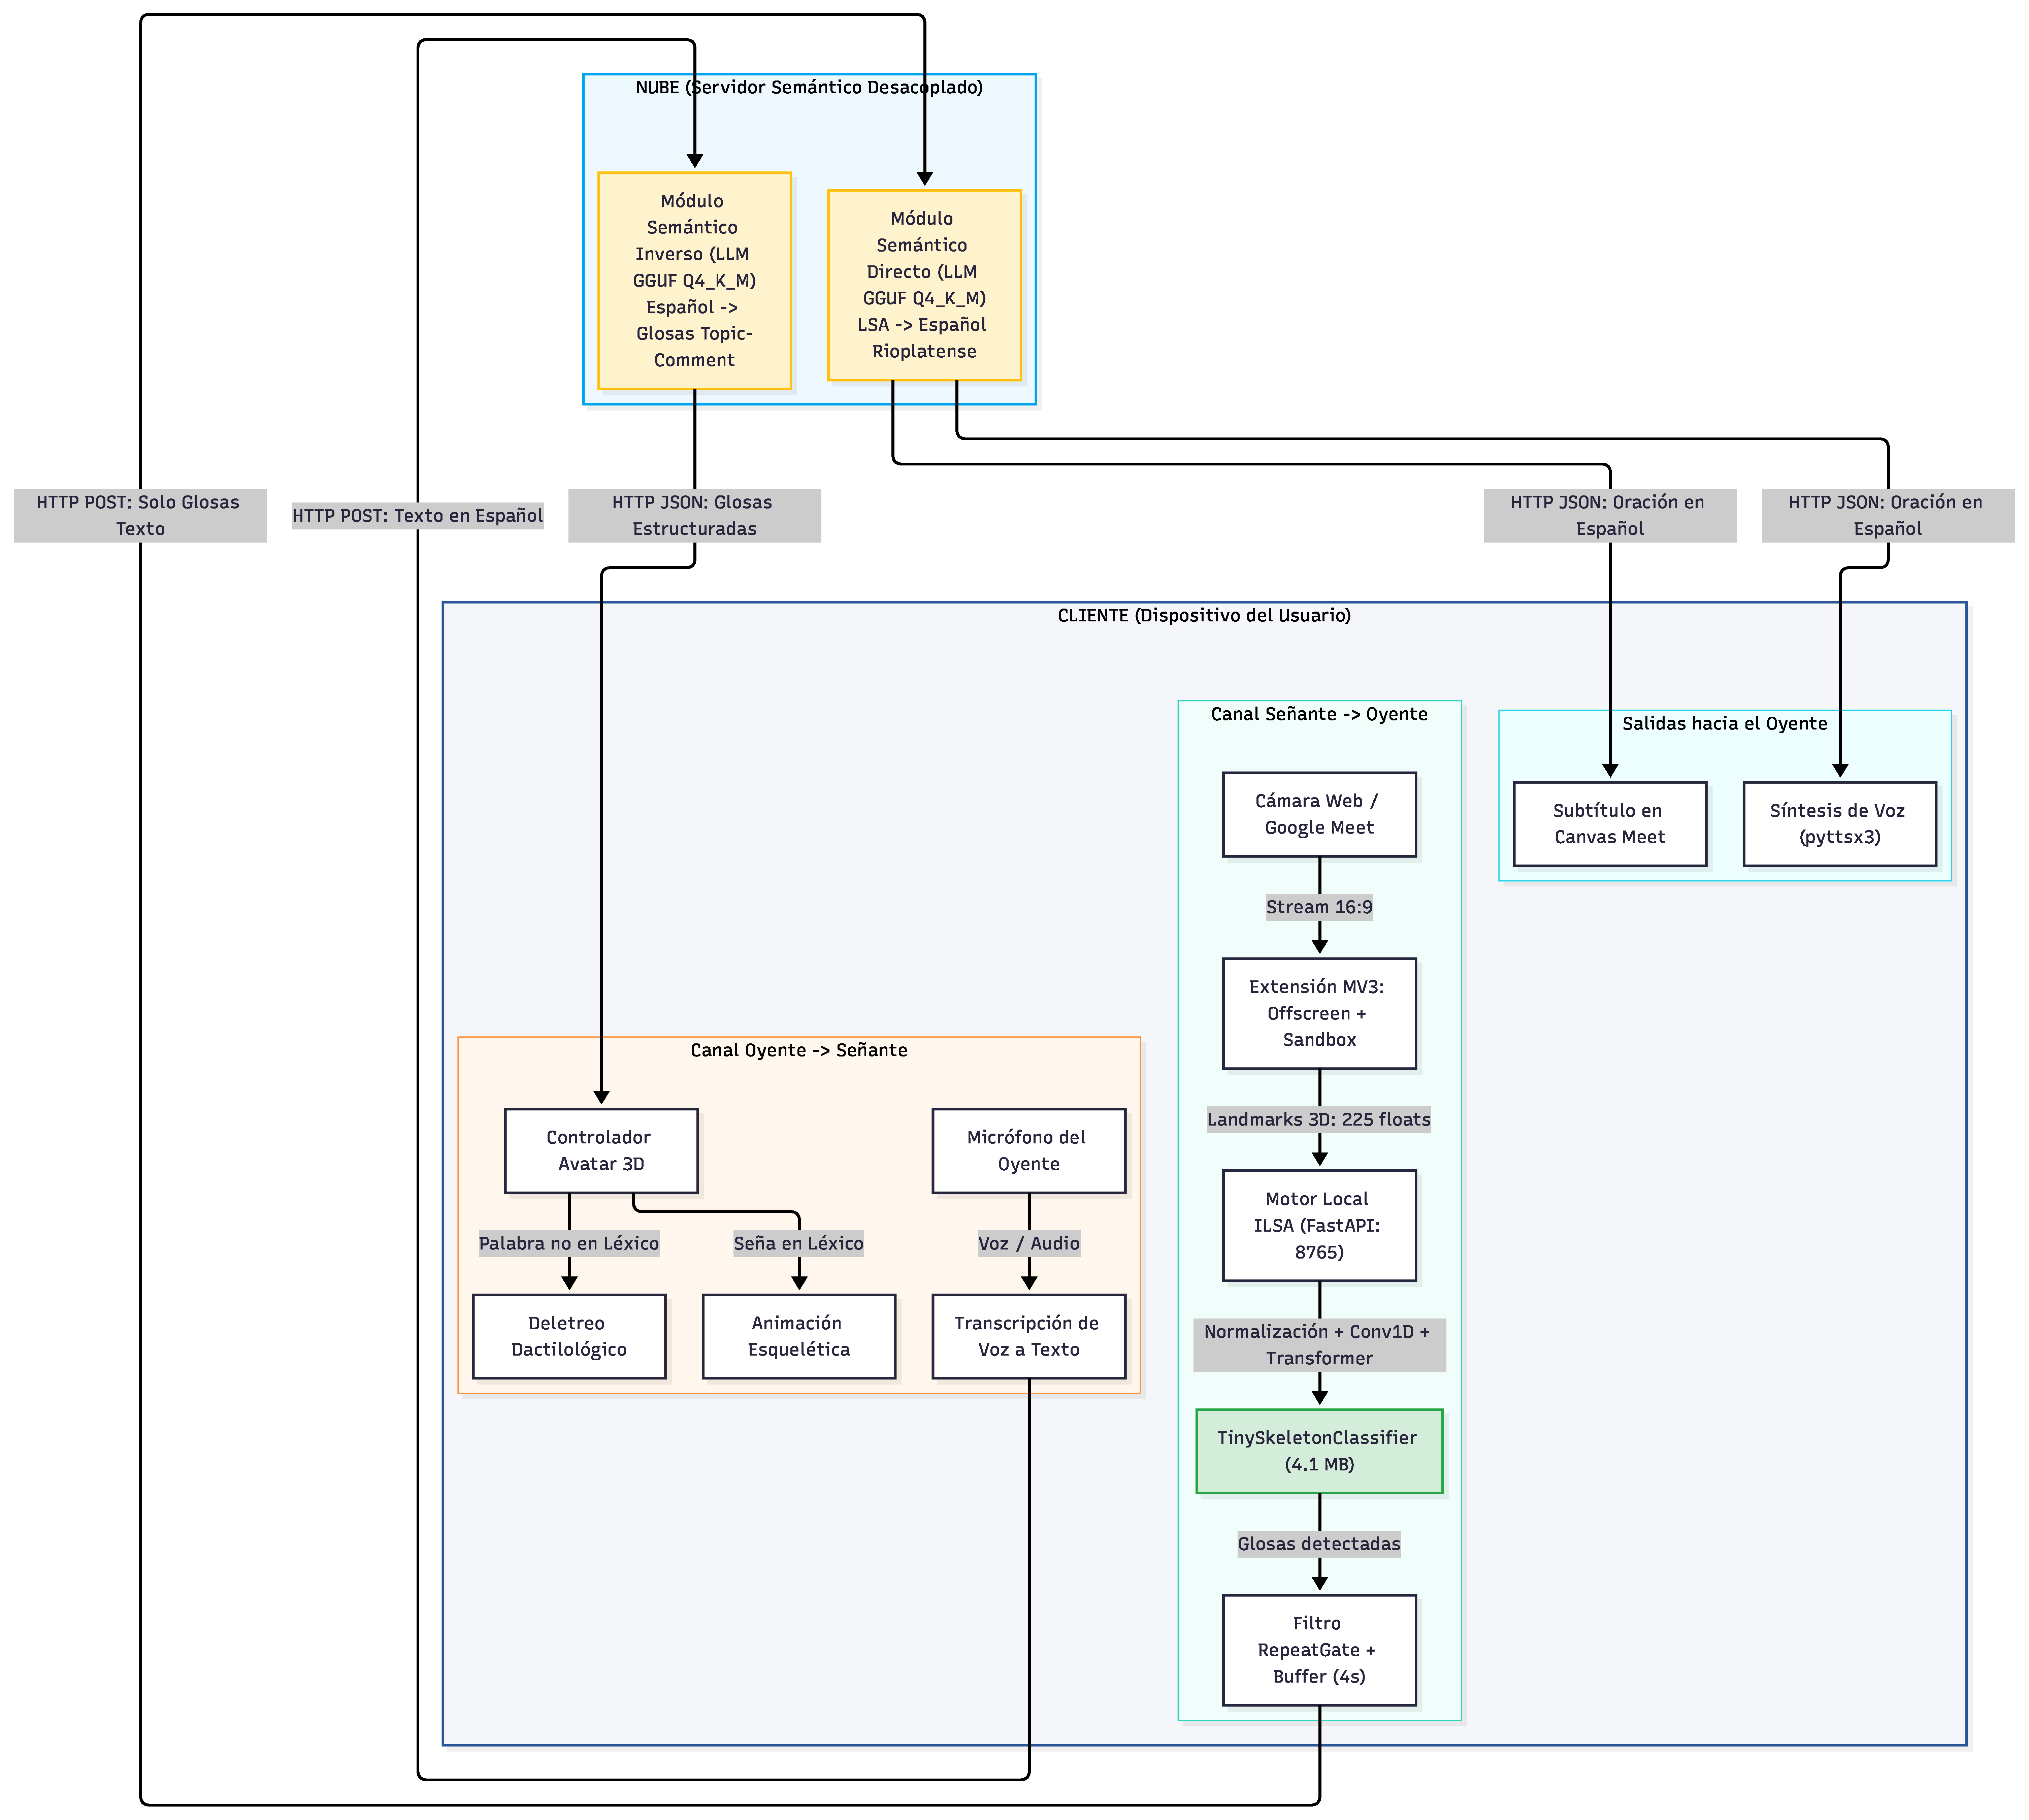
\includegraphics[width=\textwidth]{integracion/Diagrama-arquitectura.pdf}
    \caption{Arquitectura global de integración: partición entre el dispositivo cliente (captura, extracción de \textit{landmarks}, clasificación y avatar 3D) y el servidor semántico desacoplado en la nube.}
    \label{fig:diagrama_arquitectura}
\end{figure}

Para modelar la interacción temporal y la secuencia de mensajes se analizan a continuación los dos canales comunicacionales de manera independiente.

\subsubsection{Dinámica temporal del Canal Señante $\rightarrow$ Oyente (Modo Sordo)}
En la Figura~\ref{fig:secuencia_senante} se modela el ciclo de vida completo de un enunciado en LSA, desde la articulación gestual frente a la cámara web hasta la emisión de subtítulos y voz sintética hacia el interlocutor oyente.

% Figura 5.2: Secuencia señante -> oyente
\begin{figure}[H]
    \centering
    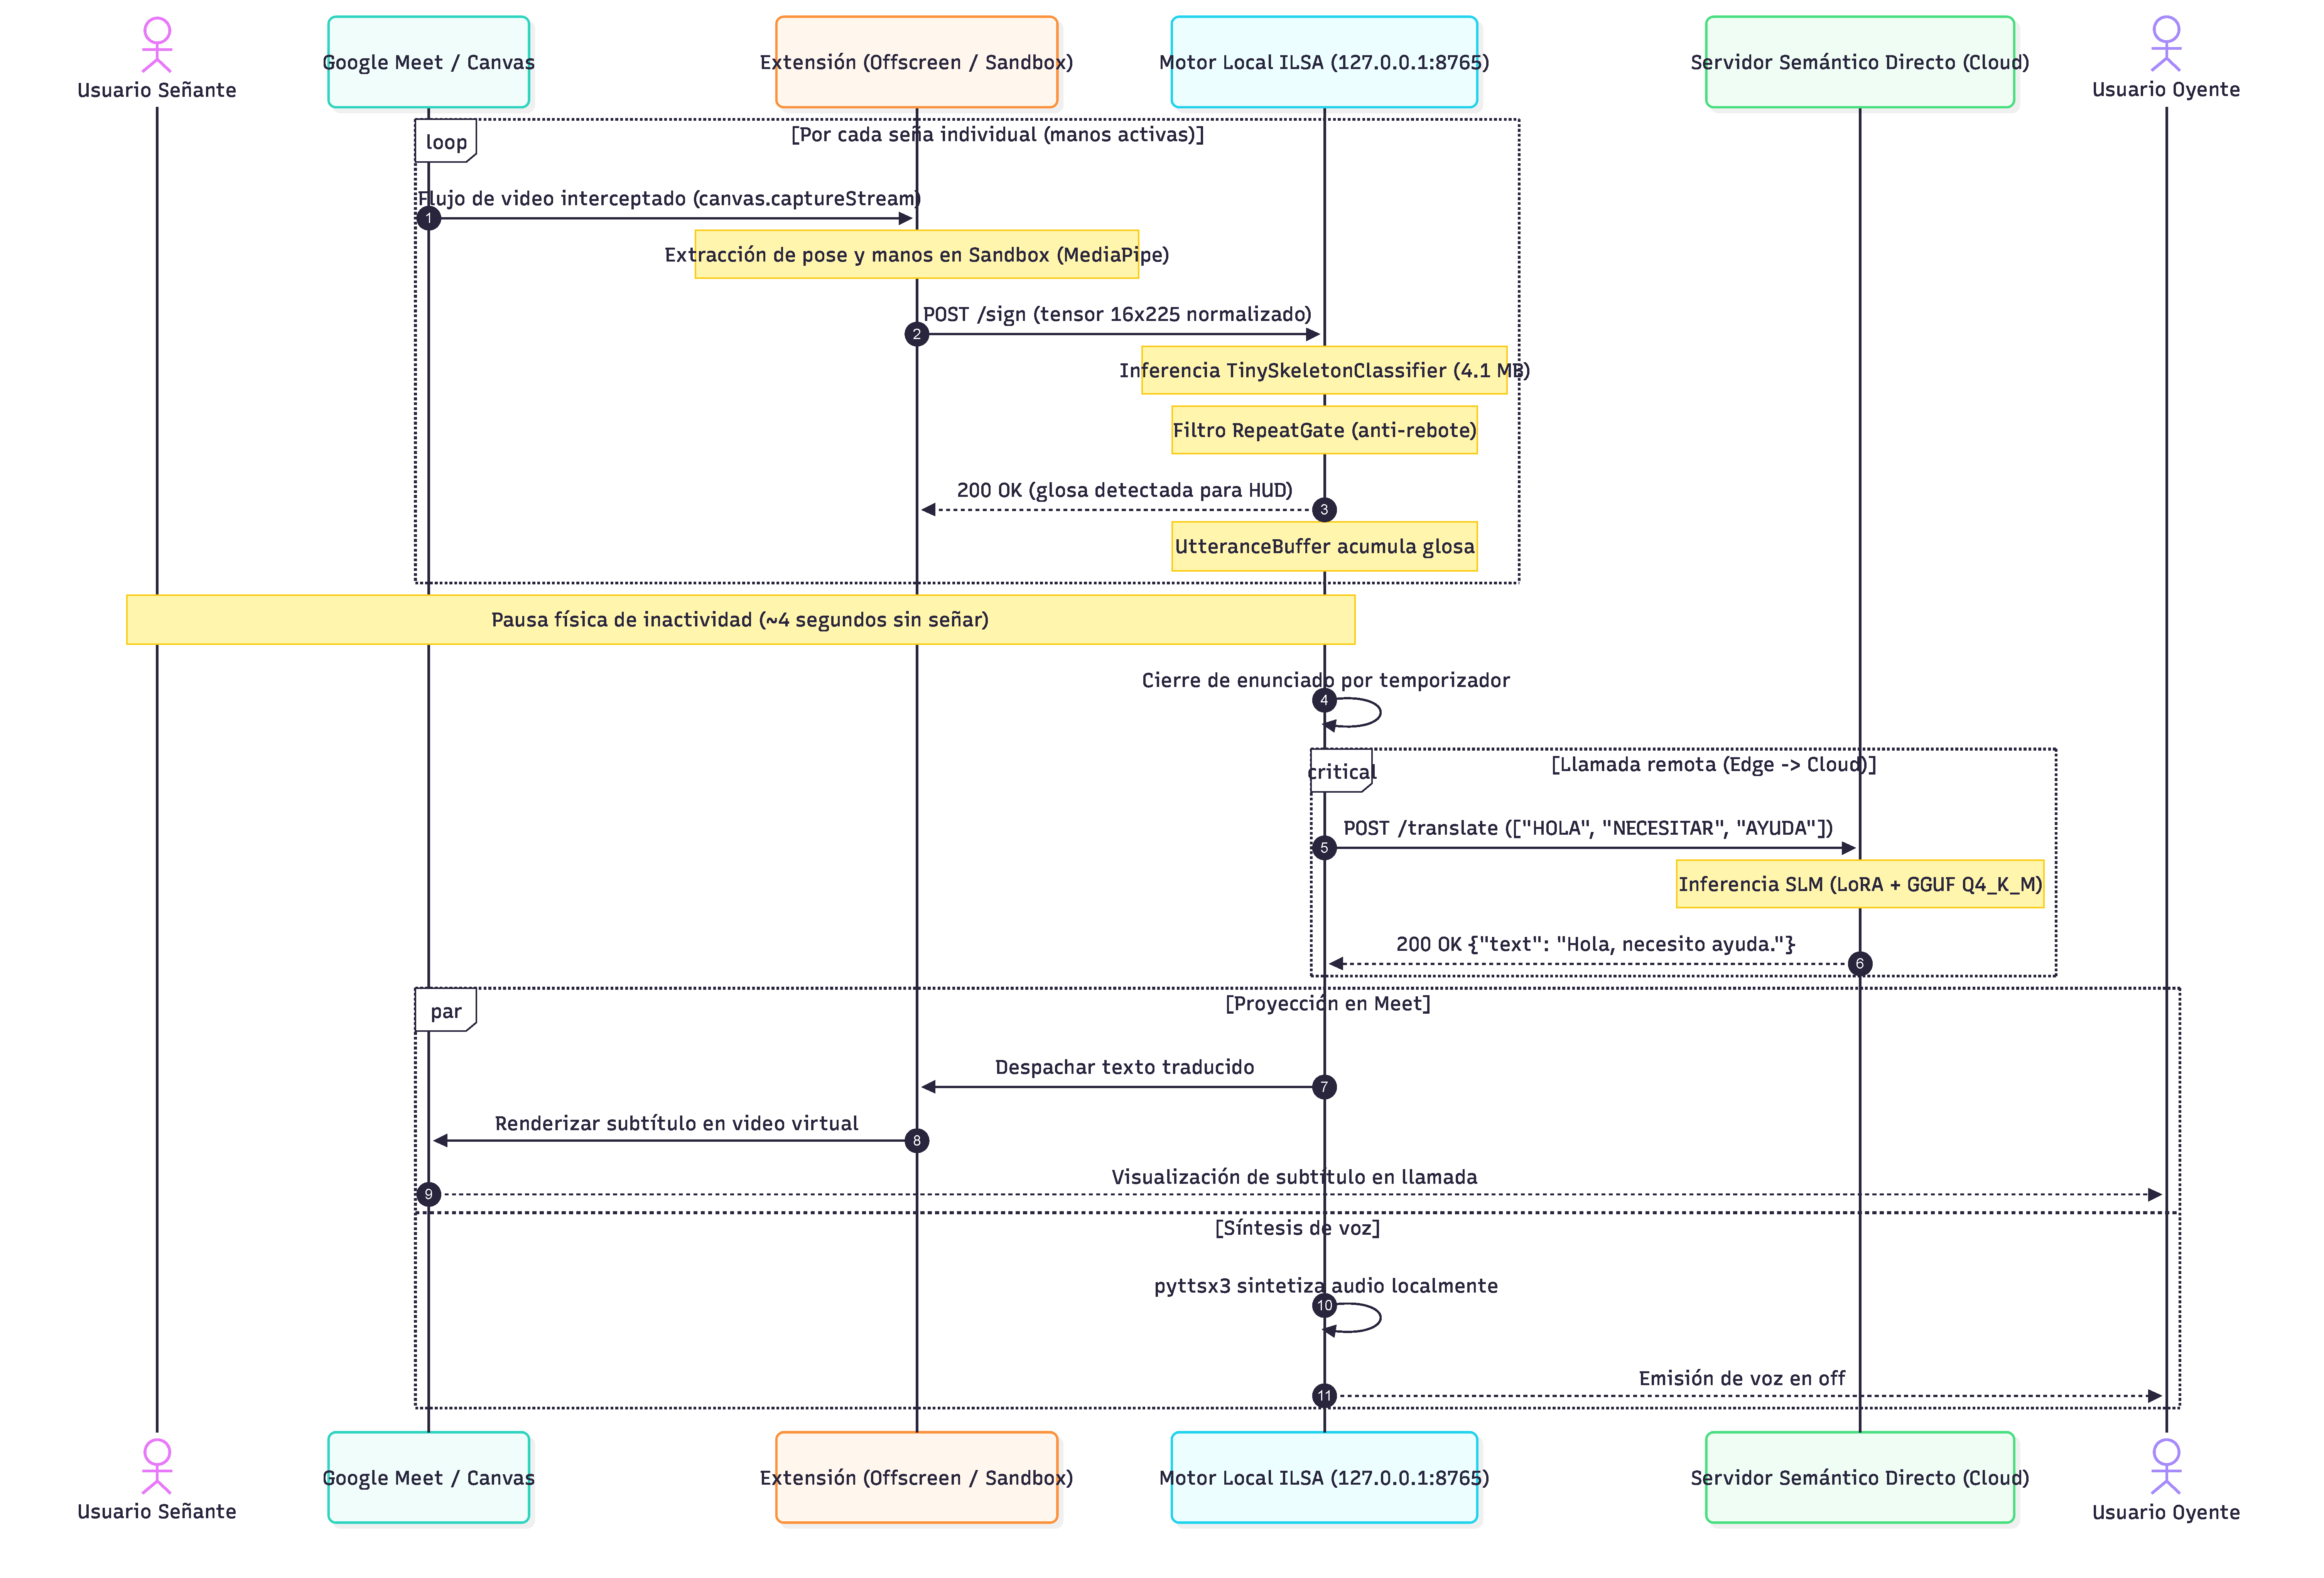
\includegraphics[width=\textwidth]{integracion/Diagrama-secuencia-senante.pdf}
    \caption{Diagrama de secuencia del Canal Señante $\rightarrow$ Oyente: bucle continuo de clasificación de señas en el borde, delimitación heurística de pausas de 4 segundos e invocación al servidor semántico remoto.}
    \label{fig:secuencia_senante}
\end{figure}

El procesamiento de este canal se rige bajo la siguiente secuencia de eventos técnicos:
\begin{enumerate}
    \item \textbf{Intercepción de video y aislamiento en la extensión:} Al activarse el sistema, la extensión intercepta la llamada a \texttt{getUserMedia} en Google Meet mediante la derivación de flujo a un elemento \texttt{<canvas>} virtual con el método \texttt{captureStream()} \parencite{w3c2024mediacapture}. Para sortear las restricciones del entorno Chrome Manifest V3 sin degradar el hilo principal de la videollamada \parencite{chrome2024manifestv3}, los cuadros de video se envían a un documento \textit{offscreen} que delega en un \textit{sandbox} aislado la inferencia de MediaPipe Holistic \parencite{google2020mediapipe}, obteniendo los 225 puntos articulares tridimensionales correspondientes a la pose y ambas manos.
    \item \textbf{Clasificación temporal continua en el motor local (ILSA):} Por cada seña aislada delimitada por la presencia y cinemática de las manos (con umbrales temporales ajustados a $\approx 0{,}9$\,s de inmovilidad o gracia de $0{,}4$\,s ante pérdidas momentáneas de seguimiento), la extensión serializa la secuencia normalizada de $16$ fotogramas y la envía mediante una petición HTTP POST (\texttt{/sign}) al servidor local FastAPI que corre en \texttt{127.0.0.1:8765}.
    % TODO: Lo mismo, chequear 2ms
    \item \textbf{Inferencia ligera y filtrado heurístico (\texttt{RepeatGate}):} El modelo neuronal \textit{TinySkeletonClassifier} ($4{,}1$\,MB) ejecuta su inferencia en CPU en menos de $2$\,ms. La predicción atraviesa la compuerta de validación \texttt{RepeatGate} \parencite{gamma1994design}, la cual aplica políticas específicas según la categoría léxica de la glosa: admite repeticiones indefinidas para dígitos numéricos, un máximo de dos apariciones consecutivas para letras individuales del alfabeto, y descarta repeticiones inmediatas en vocabulario general para suprimir rebotes del clasificador. La glosa aceptada se envía de retorno a la extensión para actualizar en tiempo real el HUD de confirmación del señante y se apila en el acumulador \texttt{UtteranceBuffer}.
    \item \textbf{Temporización y cierre de enunciado:} El acumulador monitorea la actividad gestual. Cuando el usuario retira las manos o permanece en reposo por un intervalo continuo de $4$ segundos, el temporizador de inactividad declara el cierre del enunciado.
    \item \textbf{Invocación remota al servidor semántico:} El motor local ILSA transmite exclusivamente la lista de glosas estructuradas (payload en texto de menos de $100$\,bytes) hacia el servidor semántico en la nube mediante un POST a \texttt{/translate}. El modelo de lenguaje pequeño adaptado con LoRA \parencite{hu2022lora} y cuantizado a GGUF Q4\_K\_M \parencite{gerganov2023llamacpp} resuelve la coherencia gramatical en español rioplatense.
    \item \textbf{Emisión concurrente de resultados:} La oración traducida en ILSA, se bifurca en dos salidas paralelas: se transmite a la extensión para ser dibujada como subtítulo persistente durante $8$ segundos sobre el \texttt{<canvas>} de video transmitido a Meet \parencite{w3c2024mediacapture}, y en simultáneo se envía al hilo secundario de \texttt{pyttsx3} para su reproducción sintetizada por voz hacia el oyente sin bloquear el flujo visual.
\end{enumerate}

\subsubsection{Dinámica temporal del Canal Oyente $\rightarrow$ Señante (Modo Oyente)}
En la Figura~\ref{fig:secuencia_oyente} se describe la secuencia temporal que transforma el mensaje oral del oyente en representaciones visuales comprensibles en LSA para el usuario sordo.

% Figura 5.3: Secuencia oyente -> señante
\begin{figure}[H]
    \centering
    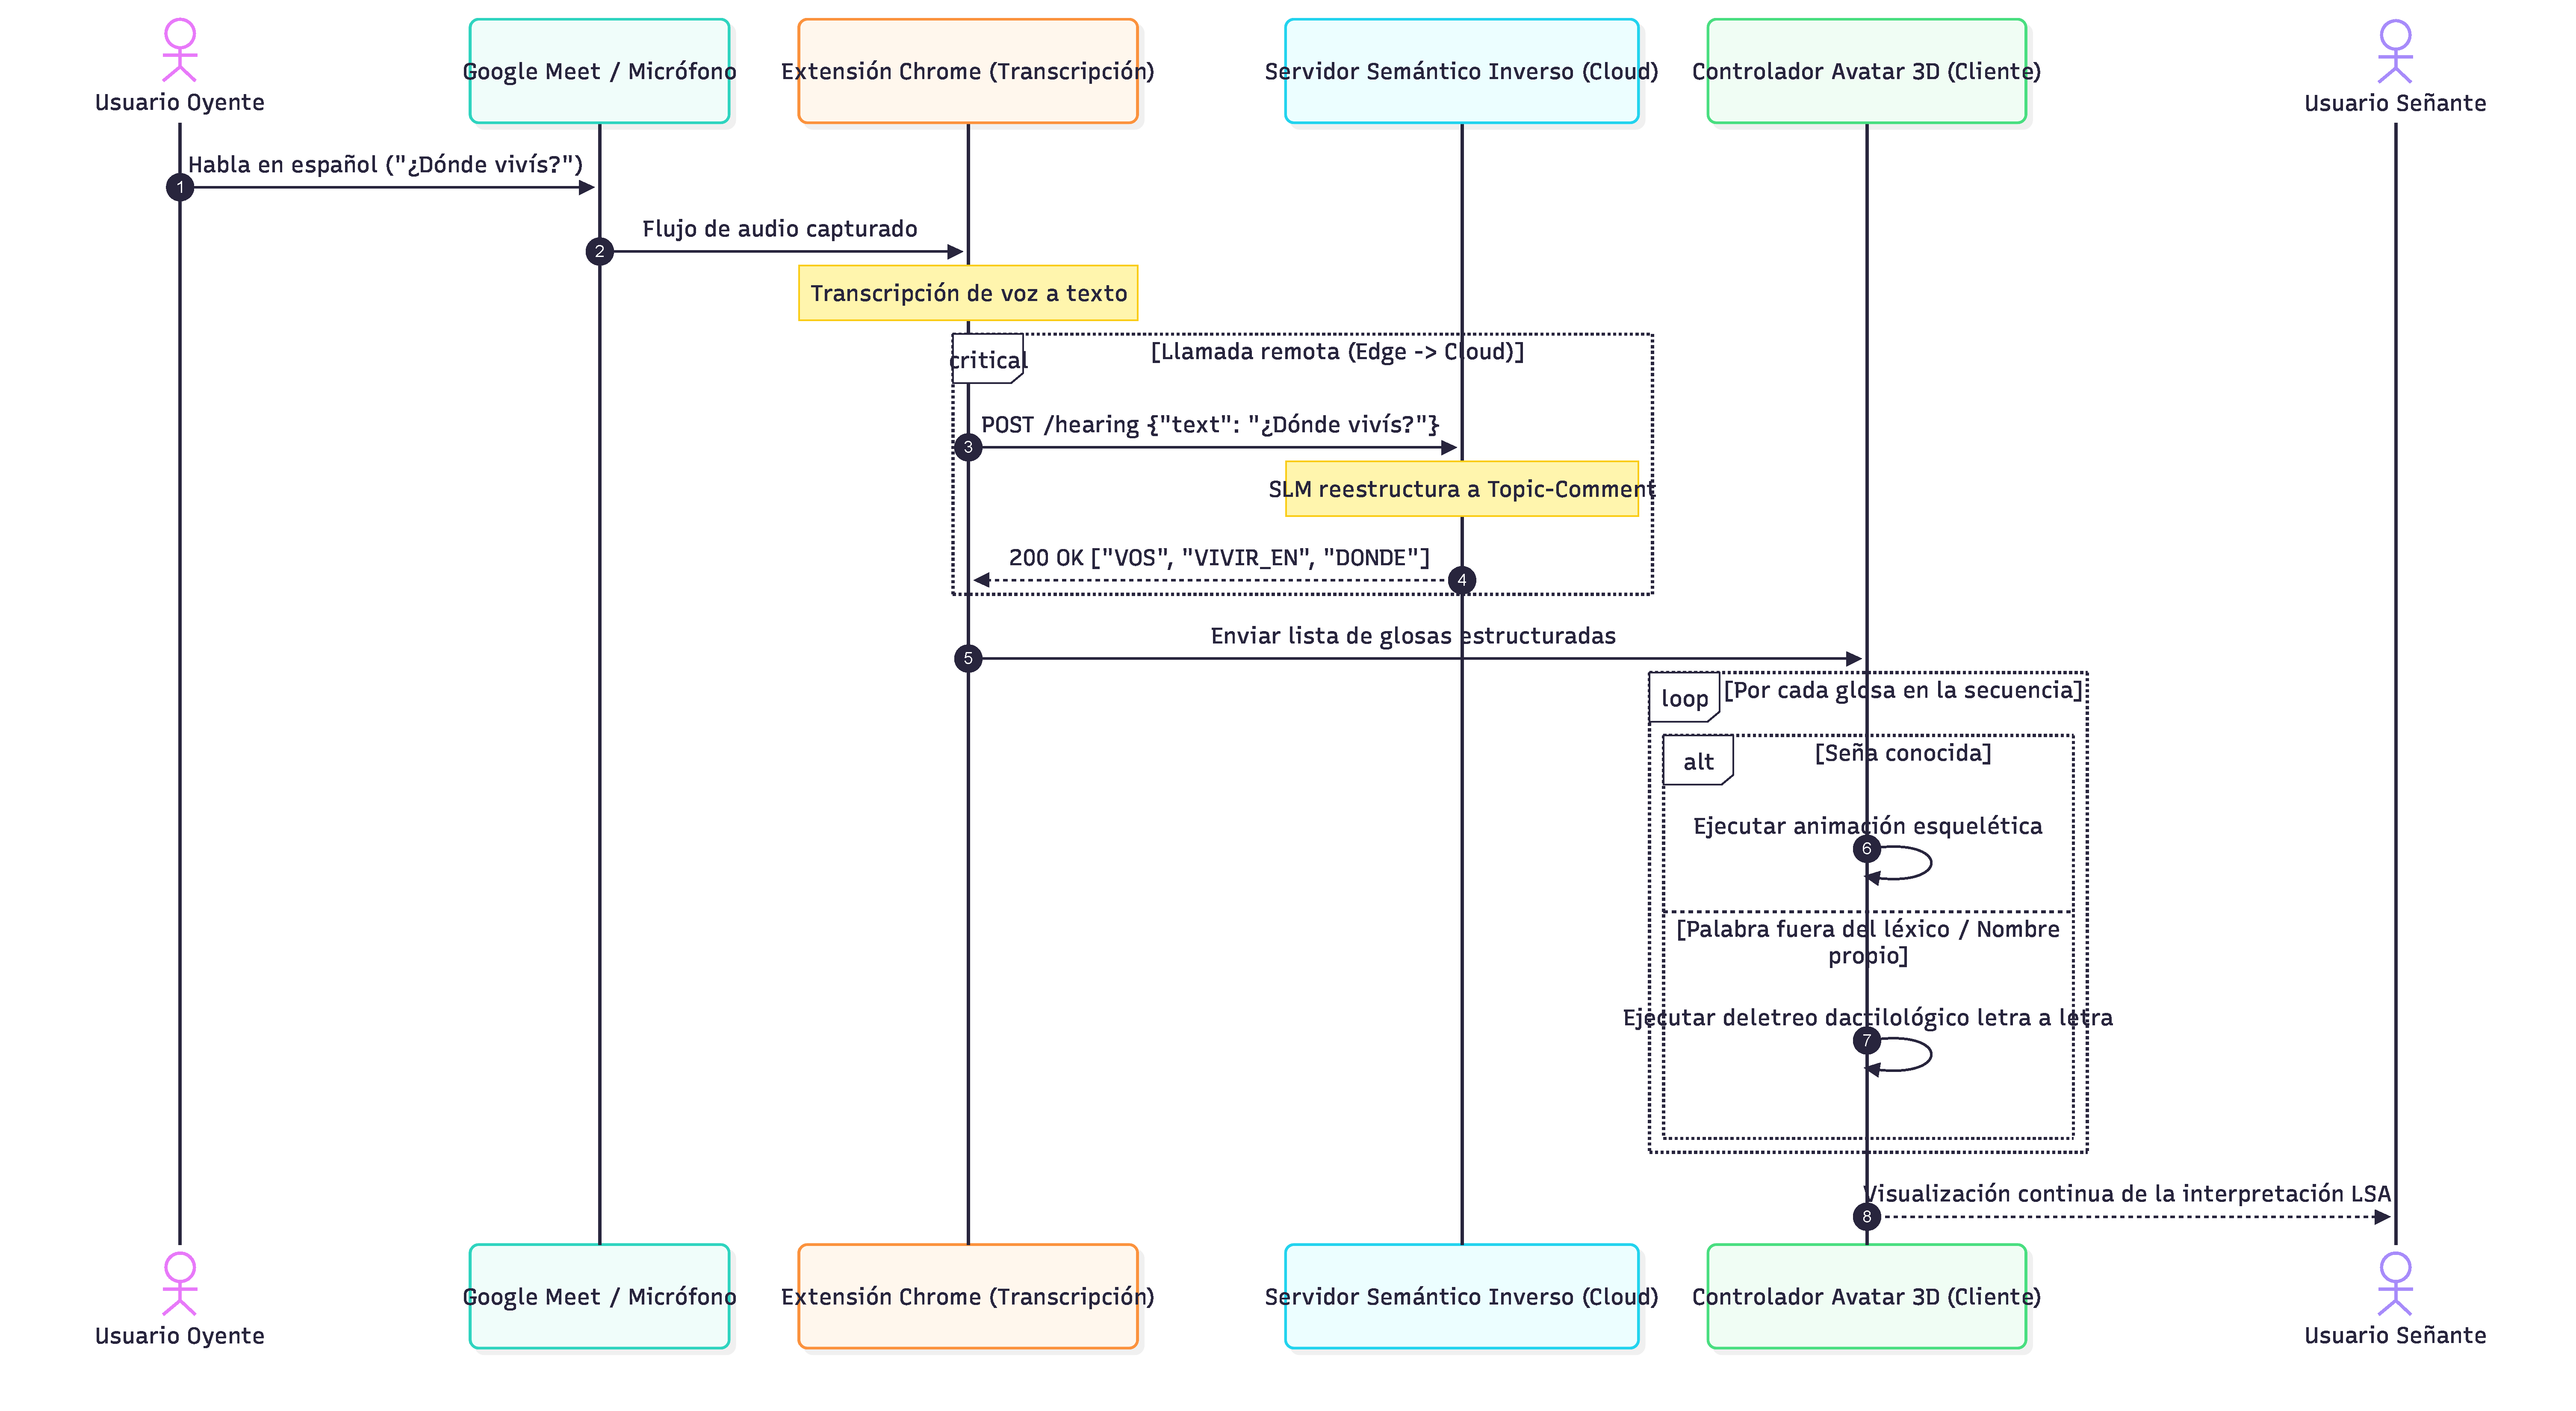
\includegraphics[width=\textwidth]{integracion/Diagrama-secuencia-oyente.pdf}
    \caption{Diagrama de secuencia del Canal Oyente $\rightarrow$ Señante: transcripción del habla, reestructuración gramatical Topic-Comment en la nube y animación o deletreo dactilológico en el cliente.}
    \label{fig:secuencia_oyente}
\end{figure}

El canal inverso se desarrolla mediante los siguientes pasos técnicos:
\begin{enumerate}
    \item \textbf{Captura y transcripción del audio:} Durante el turno del interlocutor oyente, el audio capturado en la pestaña de la videollamada es procesado por los mecanismos de reconocimiento de voz de la extensión, obteniendo la transcripción textual de la oración en español.
    \item \textbf{Estructuración semántica inversa en la nube:} La cadena textual se envía mediante HTTP POST (\texttt{/hearing}) al microservicio semántico inverso remoto. El modelo especializado aplica el conjunto de reglas aprendidas para despojar al mensaje de artículos y preposiciones abstractas, reordenando las unidades léxicas bajo la estructura gramatical \textit{Topic-Comment} propia de la LSA \parencite{massone2012curso}:
    \begin{equation}
        \text{Español: ``¿Dónde vivís?''} \quad \longrightarrow \quad \text{LSA: } [\texttt{"VOS"}, \texttt{"VIVIR\_EN"}, \texttt{"DONDE"}]
    \end{equation}
    \item \textbf{Despacho y ejecución sobre el Avatar 3D local:} La lista ordenada de glosas retorna a la extensión en el cliente, la cual invoca secuencialmente al controlador del avatar tridimensional. Para cada elemento de la secuencia:
    \begin{itemize}
        \item Si la glosa pertenece al vocabulario conocido, el motor gráfico ejecuta la interpolación esquelética correspondiente al gesto tridimensional.
        \item Si el vocablo corresponde a un término no registrado en el léxico base o a un nombre propio, el controlador acciona de manera automática la subrutina de deletreo manual dactilológico, animando letra por letra la palabra involucrada.
    \end{itemize}
    El usuario sordo visualiza de este modo la traducción continua en su lengua natural de manera sincronizada sobre la interfaz de la llamada.
\end{enumerate}

\subsection{Esquema de comunicación y contrato de interfaces (API REST)}

La integración de los componentes del sistema se articula a través de dos interfaces de programación de aplicaciones (API) basadas en el estilo arquitectónico REST, implementadas sobre el framework asíncrono FastAPI y montadas mediante servidores ASGI Uvicorn \parencite{tiangolo2018fastapi}:
\begin{enumerate}
    \item \textbf{API Local del Motor ILSA (\texttt{127.0.0.1:8765}):} Expuesta en la interfaz de bucle invertido (\textit{loopback}) del cliente, actúa como intermediaria de control entre la extensión de Chrome y los procesos locales de clasificación gestual y síntesis auditiva.
    \item \textbf{API del Servicio Semántico Remoto (\textit{Cloud}):} Microservicio desacoplado accesible a través de una URL, responsable de resolver la traducción contextual directa e inversa mediante modelos semánticos.
\end{enumerate}

\paragraph{Políticas de seguridad, CORS y enlace de red}
% TODO: Chequear si esto de q solo admite meets es valido, deberia serlo pero por las dudas
Por motivos de seguridad y privacidad estricta, el servidor local ILSA se enlaza exclusivamente a la dirección IP \texttt{127.0.0.1}, denegando peticiones originadas fuera del dispositivo cliente. Para habilitar la comunicación desde la videollamada sin vulnerar las restricciones del navegador, se implementa una política de Intercambio de Recursos de Origen Cruzado (\textit{CORS}) restrictiva que admite únicamente peticiones provenientes del origen de la plataforma (\texttt{https://meet.google.com}), orígenes con el esquema de extensión del navegador (\texttt{chrome-extension://*}) y \texttt{localhost}.

\subsubsection{Contratos de la API Local ILSA}
La interacción entre la extensión y el motor local se rige por contratos tipados mediante esquemas Pydantic \parencite{tiangolo2018fastapi}. La Tabla~\ref{tab:endpoints_ilsa} resume los principales endpoints provistos por el motor local.
\begin{table}[H]
\centering
\small
\renewcommand{\arraystretch}{1.25}
\setlength{\tabcolsep}{4.5pt}
\caption{Endpoints principales de la API local del motor ILSA (127.0.0.1:8765)}
\label{tab:endpoints_ilsa}
\begin{tabularx}{\textwidth}{@{}>{\bfseries}l >{\ttfamily}l >{\raggedright\arraybackslash\hsize=0.55\hsize}X >{\raggedright\arraybackslash\hsize=1.45\hsize}X@{}}
\toprule
Método & \textrm{\textbf{Ruta}} & \textbf{Esquema / Parámetros} & \textbf{Descripción y Comportamiento} \\
\midrule
GET & /health & Ninguno & Monitoreo del estado operativo del clasificador y conectividad con el traductor semántico. \\
\addlinespace[3pt]
GET & /state & Ninguno & Devuelve las glosas acumuladas en el búfer temporal y el último texto traducido. \\
\addlinespace[3pt]
POST & /session & Session\-Start\-Request & Inicia una sesión de señado configurando la lateralidad (\texttt{left\_handed: bool}). \\
\addlinespace[3pt]
POST & /sign & SignPayload & Ingesta una lista de 16 fotogramas con 225 coordenadas articulares normalizadas; ejecuta el clasificador y el filtro RepeatGate. \\
\addlinespace[3pt]
POST & /activity & Ninguno & Notifica actividad cinemática para resetear el temporizador de cierre de enunciado. \\
\addlinespace[3pt]
POST & /utterance/end & Ninguno & Cierra forzosamente el enunciado actual, despacha las glosas acumuladas al traductor y vacía el búfer. \\
\addlinespace[3pt]
POST & /conversation/clear & Ninguno & Reinicia el contexto conversacional de turnos cruzados. \\
\bottomrule
\end{tabularx}
\end{table}

% No habria q poner tambien que formato tiene SessionStartRequest??
\paragraph{Estructura de la carga de entrada para clasificación (\texttt{/sign})}
El endpoint \texttt{/sign} consume un objeto JSON con la secuencia cinemática procesada en el navegador:
\begin{verbatim}
{
  "frames": [
    [0.012, -0.451, ..., 0.128],   // 225 flotantes del fotograma 0
    ...
    [-0.005, -0.442, ..., 0.119]   // 225 flotantes del fotograma 15
  ],
  "source_fps": 30.0
}
\end{verbatim}
En respuesta, el motor valida el gesto y devuelve un objeto de confirmación que alimenta el visor de estado (HUD) de la extensión:
\begin{verbatim}
{
  "status": "accepted",
  "gloss": "HOLA",
  "confidence": 0.942,
  "top3": [
    {"gloss": "HOLA", "prob": 0.942},
    {"gloss": "CHAU", "prob": 0.031},
    {"gloss": "VER",  "prob": 0.015}
  ],
  "utterance_closed": false
}
\end{verbatim}

\subsubsection{Contratos de la API del Servicio Semántico Remoto}
El microservicio en la nube centraliza la inferencia del modelo de lenguaje a través de dos rutas, resumidas en la Tabla~\ref{tab:endpoints_semantico}.

\begin{table}[h!]
\centering
\small
\renewcommand{\arraystretch}{1.4}
\setlength{\tabcolsep}{5pt} % Reduce levemente el espacio entre columnas para evitar desbordes
\begin{tabularx}{\textwidth}{|>{\raggedright\arraybackslash\bfseries}p{3.5cm}|c|>{\raggedright\arraybackslash}X|>{\raggedright\arraybackslash}X|}
\hline
Identificador & \multicolumn{3}{l|}{\textbf{CU-01: Conversar con otra persona}} \\
\hline
Actor principal & \multicolumn{3}{l|}{Usuario señante} \\
\hline
Precondiciones & \multicolumn{3}{l|}{El usuario debe estar unido a una llamada.} \\
\hline
Postcondiciones & \multicolumn{3}{p{\dimexpr\textwidth-3.5cm-6\tabcolsep-4\arrayrulewidth\relax}|}{El usuario no señante es capaz de leer/escuchar lo que el usuario señante le dice.} \\
\hline
\multirow{3}{=}{Escenario Principal de éxito (flujo básico)} 
 & & \textbf{Usuario señante} & \textbf{Sistema} \\
\cline{2-4}
 & \textbf{1} & Realiza las señas correspondientes a lo que quiere comunicar. & \\
\cline{2-4}
 & \textbf{2} & & El Sistema procesa el búfer con las señas, extrae los landmarks, interpreta cada gesto y envía la secuencia al módulo semántico, el cual traduce y muestra por pantalla la oración resultante. \\
\hline
Extensiones & \multicolumn{3}{l|}{---} \\
\hline
Requisitos especiales & \multicolumn{3}{l|}{---} \\
\hline
\end{tabularx}
\end{table}

\paragraph{Contrato del Canal Directo (\texttt{/translate})}
La petición generada por el motor local hacia el servidor remoto encapsula las glosas detectadas y el historial deslizante:

% TODO: Esto funciona asi? Me refiero a lo de que manda el texto en history
\begingroup
\small
\begin{verbatim}
// Solicitud POST /translate
{
  "glosses": ["AHORA_HOY", "YO", "BIEN"],
  "history": [
    {"role": "hearing", "text": "¿Cómo estás hoy?"}
  ]
}

// Respuesta 200 OK
{
  "spanish": "Hoy estoy bien.",
  "model_used": "llama-3.2-1b-instruct-lsa-q4_k_m",
  "inference_time_ms": 348.3
}
\end{verbatim}
\endgroup
\paragraph{Contrato del Canal Inverso (\texttt{/hearing})}
En sentido inverso, el texto transcripto de la voz del oyente se remite al modelo inverso para su desarticulación gramatical:
\begin{verbatim}
// Solicitud POST /hearing
{
  "text": "¿Dónde vivís actualmente?"
}

// Respuesta 200 OK
{
  "glosses": ["VOS", "VIVIR_EN", "DONDE"],
  "inference_time_ms": 337.7
}
\end{verbatim}

Este desacoplamiento contractual garantiza una delimitación de responsabilidades limpia: el motor cliente no depende de la arquitectura interna ni de los pesos del modelo de lenguaje que atiende en la API remota, requiriendo únicamente el cumplimiento estricto del esquema de intercambio JSON.

\section{Subsistema de reconocimiento gestual (Clasificador)}
\subsection{Captura e ingesta de video con MediaPipe Holistic}
\subsection{Normalización geométrica y corrección de distorsión de relación de aspecto}
\subsection{Preprocesamiento: recorte temporal, submuestreo e interpolación}
\subsection{Arquitectura neuronal TinySkeletonClassifier (Conv1D + transformer + attention pooling)}
\subsection{Segmentación continua y políticas anti-rebote (RepeatGate)}

\section{Subsistema de traducción semántica bidireccional}
\subsection{Canal directo (\texorpdfstring{LSA $\rightarrow$ Español}{LSA -> Español}): fine-tuning LoRA y loss masking}

El canal directo tiene como propósito transformar secuencias de glosas aisladas provenientes del clasificador gestual en oraciones sintáctica y semánticamente correctas en español rioplatense natural. A diferencia de una correspondencia léxica término a término, este módulo debe inferir artículos, preposiciones, flexiones verbales y terminaciones de género que no se encuentran explicitas en la estructura de entrada de las señas.

\paragraph{Estructuración léxica y reglas de traducción}
En la fase de refinamiento se suprimieron los ejemplos demostrativos fijos (\textit{few-shots}) en el prompt, optando por un \textit{system prompt} compacto y estricto. Sobre el vocabulario formalizado de 100 clases, las directivas lingüísticas integradas regulan:
\begin{itemize}
    \item \textbf{Marcadores temporales y flexión verbal:} Las glosas temporales iniciales condicionan la conjugación de los verbos subsiguientes. Glosas como \texttt{PASADO} o \texttt{AYER} obligan al uso de pretérito, \texttt{FUTURO} rige el tiempo futuro y la ausencia de marcador temporal se traduce por defecto en presente del indicativo.
    \item \textbf{Resolución de género en parentescos mediante dactilología:} De acuerdo con los estudios de morfología en LSA \parencite{massone1993numero},los sustantivos no suelen tener una terminación fija para masculino o femenino. Por eso, en los términos de parentesco, se adoptó la combinación de la seña base con las letras dactilológicas \texttt{[A]} u \texttt{[O]} para marcar explícitamente el género femenino o masculino:
    \begin{align*}
        \texttt{["HIJO", "A"]} &\quad\longrightarrow\quad \text{``Hija''} \\
        \texttt{["HIJO", "O"]} &\quad\longrightarrow\quad \text{``Hijo''} \\
        \texttt{["HERMANO", "A"]} &\quad\longrightarrow\quad \text{``Hermana''} \\
        \texttt{["ESPOSO", "A"]} &\quad\longrightarrow\quad \text{``Esposa''}
    \end{align*}
    El modelo semántico interpreta esta letra añadida y ajusta la terminación de la palabra en español. Ante la ausencia de una marca explícita, genera la forma masculina o neutra por defecto.
    \item \textbf{Fórmulas de interacción, auxilio y cortesía:} La inclusión de glosas como \texttt{AYUDAR} y \texttt{GRACIAS} permite estructurar pedidos de auxilio y fórmulas de interacción esenciales en situaciones de emergencia o diálogo cotidiano (e.g., \texttt{["GRACIAS"]} $\longrightarrow$ \textit{``Gracias''}; \texttt{["VOS", "YO", "AYUDAR", "PODER"]} $\longrightarrow$ \textit{``¿Me podés ayudar?''}; \texttt{["YO", "VOS", "AYUDAR"]} $\longrightarrow$ \textit{``Te ayudo''}).    
    \item \textbf{Uso de posesivos:} Las glosas \texttt{MIO} y \texttt{TUYO} se traducen de forma natural en español según el objeto que acompañen (por ejemplo, \textit{«mi documento»} o \textit{«tu casa»}).
\end{itemize}

\paragraph{Mecanismo de Loss Masking (\texttt{train\_on\_responses\_only}).}
En el entrenamiento estándar de modelos sobre pares de instrucción y respuesta, la función de pérdida por entropía cruzada se computa sobre la totalidad de los tokens de la secuencia. Esto obliga a la red a predecir tanto las instrucciones del sistema como las glosas de entrada.

Para optimizar el uso del gradiente, se implementó la técnica de enmascaramiento de pérdida (\textit{loss masking}) mediante la directiva \texttt{train\_on\_responses\_only} \parencite{huggingface2024transformers}. En el cálculo de la función objetivo, los tokens correspondientes al prompt del sistema y a la lista de glosas son etiquetados con el identificador $-100$, ignorándolos en la optimización, donde el cómputo del error recae exclusivamente sobre los $M$ tokens de la oración final en español condicionada por el contexto. De este modo, la actualización de pesos se concentra por completo en la fluidez y precisión gramatical del texto generado.

% TODO: Lo dejamos? No se si es necesario la explicacion con ecuaciones de como funciona Lora
\paragraph{Adaptación LoRA profunda y proyecciones de vocabulario.}
La adaptación eficiente de bajo rango (\textit{LoRA}) descompone las matrices de pesos preentrenadas $\mathbf{W}_0 \in \mathbb{R}^{d \times k}$ en dos matrices entrenables $\mathbf{B} \in \mathbb{R}^{d \times r}$ y $\mathbf{A} \in \mathbb{R}^{r \times k}$ (donde $r \ll \min(d, k)$), actualizando los pesos según $\mathbf{W} = \mathbf{W}_0 + \frac{\alpha}{r}(\mathbf{B}\mathbf{A})$ \parencite{hu2022lora}.

Además de inyectar adaptadores en las matrices de proyección de atención convencionales (\texttt{q\_proj}, \texttt{k\_proj}, \texttt{v\_proj}, \texttt{o\_proj}), la arquitectura del traductor incorporó de forma deliberada adaptadores LoRA sobre los extremos del modelo:
\begin{itemize}
    \item \textbf{\texttt{embed\_tokens}:} Adapta la capa de embedding de entrada para que las 100 glosas en mayúsculas se proyecten en representaciones semánticas que capturen la estructura de unidades de lengua de señas.
    \item \textbf{\texttt{lm\_head}:} Ajusta la capa lineal de desproyección final hacia el vocabulario, facilitando que la red asigne probabilidades a artículos, preposiciones y terminaciones verbales del español rioplatense.
\end{itemize}

\paragraph{Configuración hiperparamétrica del entrenamiento}
Para estabilizar el proceso de optimización frente al volumen acotado del dataset se adoptaron los siguientes hiperparámetros de entrenamiento:
\begin{itemize}
    \item Parámetros de adaptación LoRA: rango de descomposición $r = 16$ y factor de escala $\alpha = 32$ (incrementado para otorgar mayor ponderación relativa a las matrices residuales adaptadas) \parencite{hu2022lora}.
    \item Tasa de aprendizaje (\textit{learning rate}): valor base de $\eta = 5 \times 10^{-5}$ con decaimiento coseno suave (\textit{cosine learning rate scheduler}).
    \item Esquema de épocas y lotes: entrenamiento establecido en 10 épocas completas con un tamaño de lote efectivo de 4 muestras procesadas mediante acumulación de gradientes.
\end{itemize}

\subsection{Canal inverso (\texorpdfstring{Español $\rightarrow$ LSA}{Español -> LSA}): estructuración gramatical topic-comment}

El canal inverso tiene como propósito resolver la interpretación simétrica del mensaje: transformar el texto en español oral o escrito emitido por el interlocutor oyente hacia una secuencia estructurada de glosas sintácticas. Al igual que en el canal directo, esta operación no admite un reemplazo directo palabra por palabra, ya que exige desarmar la estructura de la oración en español y reordenar las palabras según la gramática de la LSA.

\paragraph{Asimetría de dominios y desafío de generalización abierta.}
Durante las primeras iteraciones se asumió que el modelo inverso podía entrenarse invirtiendo simétricamente el corpus paralelo utilizado para el canal directo. Sin embargo, la experimentación reveló una asimetría metodológica crítica entre ambos extremos comunicacionales:
\begin{itemize}
    \item \textbf{Canal directo (Dominio cerrado):} La entrada está rígidamente acotada por construcción a las 100 clases que el clasificador visual es capaz de reconocer. El modelo solo debe aprender a combinar e infleccionar ese léxico cerrado hacia el español.
    \item \textbf{Canal inverso (Dominio abierto):} La entrada corresponde al habla o texto libre del interlocutor oyente, el cual contiene un léxico virtualmente infinito: sinónimos no contemplados, giros coloquiales, tiempos compuestos y estructuras sintácticas complejas.
\end{itemize}
Entrenar el modelo con un conjunto limitado a oraciones espejo construidas únicamente con las 100 palabras provocaba un sobreajuste severo: ante vocablos no previstos, nombres propios o frases indirectas del oyente, el modelo colapsaba o generaba alucinaciones intentando forzar glosas conocidas.

\paragraph{Metodología de refinamiento impulsada por fallos (\textit{Failure-Driven Loop}).}
Para sortear esta limitación sin incurrir en costos inabordables de anotación manual, se implementó un ciclo iterativo de ingeniería y aprendizaje activo:
\begin{enumerate}
    \item \textbf{Entrenamiento inicial:} Ajuste con LoRA sobre el corpus inverso de partida.
    \item \textbf{Evaluación con casos límite:} Pruebas automáticas sobre oraciones variadas para evaluar la flexibilidad del modelo ante sinónimos y estructuras complejas en español.
    \item \textbf{Análisis de fallas recurrentes:} Identificación de fallas repetidas, como dejar preposiciones que no se señan, ubicar mal las preguntas al inicio o invertir el orden de la acción.
    \item \textbf{Corrección del dataset:} Agregado de nuevos pares de oraciones enfocados puntualmente en los patrones que causaban error.
    \item \textbf{Reentrenamiento y control:} Reentrenamiento del adaptador y comparación cuantitativa de métricas sintácticas (BLEU, ROUGE-L) y latencia.
\end{enumerate}

\paragraph{Estructuración gramatical y reglas del System Prompt.}
El comportamiento del modelo de lenguaje se rige mediante un \textit{system prompt} estricto que instruye al modelo a responder exclusivamente con glosas léxicas en mayúsculas, separadas por espacios, sin signos de puntuación adicionales ni artículos en español. Las directivas morfosintácticas integradas exigen:
\begin{enumerate}
    \item \textbf{Supresión de elementos no señados:} Eliminación sistemática de artículos determinados e indeterminados (``el'', ``la'', ``los'', ``un''), cópulas abstractas (``ser'', ``estar'') y preposiciones gramaticales vacías (``de'', ``a'', ``con'') \parencite{massone2012curso}.
    \item \textbf{Orden canónico Topic-Comment:} Reestructuración pragmática de la oración siguiendo el orden jerárquico de la LSA \parencite{massone2012curso}:
    \begin{equation}
    \begin{aligned}
        \text{Orden LSA} = &\ \text{TIEMPO} \longrightarrow \text{LUGAR} \longrightarrow \text{SUJETO} \longrightarrow \text{OBJETO/SUST.} \\
        &\longrightarrow \text{VERBO} \longrightarrow \text{PREGUNTA / NEGACIÓN}
    \end{aligned}
    \end{equation}
    \item \textbf{Marcación temporal inicial:} Las referencias temporales explícitas o deducidas de la conjugación se extraen y posicionan obligatoriamente en el arranque del enunciado mediante glosas como \texttt{PASADO}, \texttt{FUTURO}, \texttt{AYER} o \texttt{AHORA\_HOY}.
    \item \textbf{Explicitación pronominal:} En español es frecuente el sujeto tácito; la LSA requiere la presencia de los pronombres de primera y segunda persona (\texttt{YO}, \texttt{VOS}), por lo que el modelo infiere y explicita estos índices cuando están elididos (e.g., \textit{``Tengo un cuchillo''} $\rightarrow$ \texttt{["YO", "CUCHILLO", "TENER"]}) \parencite{massone1993numero}.
    \item \textbf{Cierre con negación e interrogativos:} Las partículas interrogativas (\texttt{QUÉ}, \texttt{DÓNDE}, \texttt{QUIÉN}, \texttt{CUÁNDO}, \texttt{CUÁNTOS}) y los marcadores de polaridad negativa (\texttt{NO}) se desplazan a la posición final de la proposición, actuando como operadores de cierre sintáctico \parencite{massone2012curso}.
\end{enumerate}

Este procesamiento asegura que la secuencia de glosas resultante refleje fielmente la organización espacial y mental de la lengua de señas antes de ser despachada al controlador del avatar 3D.

\subsection{Optimización de inferencia: formato GGUF y cuantización a 4 bits}

La integración de SLMs en una arquitectura interactiva orientada a videollamadas impone restricciones severas sobre la memoria volátil y la latencia de respuesta por token. Ejecutar modelos de lenguaje en precisión estándar de punto flotante de 16 bits (\texttt{float16}) demanda entre 2{,}5\,GB y más de 6\,GB de memoria VRAM/RAM dedicada únicamente a los pesos, lo cual resulta prohibitivo para entornos locales compartidos con decodificación de video WebRTC. Para garantizar una inferencia rápida y de bajo consumo, se implementó un pipeline de exportación y compresión post-entrenamiento hacia el formato unificado GGUF (\textit{GPT-Generated Unified Format}) ejecutado mediante el runtime \texttt{llama.cpp} \parencite{gerganov2023llamacpp}.

\paragraph{Consolidación de adaptadores y exportación.}
Una vez finalizado el ajuste fino supervisado del modelo con adaptadores LoRA, los pesos residuales de bajo rango no se cargan de manera dinámica en el entorno de producción. En su lugar, se realiza una fusión determinista (\textit{weight merging}) aplicando la rutina \texttt{save\_pretrained\_gguf}:
\begin{equation}
    \mathbf{W}_{\text{final}} = \mathbf{W}_0 + \frac{\alpha}{r} (\mathbf{B}\mathbf{A})
\end{equation}
donde $\mathbf{W}_0$ corresponde a los tensores base preentrenados del SLM (e.g., Llama 3.2 1B \parencite{dubey2024llama3} o Qwen2.5 \parencite{qwen2024qwen25}) y $\mathbf{B}\mathbf{A}$ representa la descomposición adaptada de las proyecciones de atención y capas de vocabulario (\texttt{embed\_tokens} y \texttt{lm\_head}). Esta fusión consolida la parametrización en un archivo único libre de sobrecargas de enlace en tiempo de ejecución.

\paragraph{Mecánica de cuantización Q4\_K\_M}
A partir del binario consolidado en precisión de 16 bits, se aplica el algoritmo de cuantización por bloques \texttt{Q4\_K\_M} provisto por \texttt{llama.cpp} \parencite{gerganov2023llamacpp, frantar2022gptq}. A diferencia de los métodos uniformes tradicionales donde todos los parámetros se reducen a la misma precisión, la estrategia de k-cuants (\textit{k-quants}) adopta un esquema heterogéneo basado en la sensibilidad de cada estructura neuronal:
\begin{itemize}
    \item \textbf{Tensores de auto-atención y activación (\texttt{q\_proj}, \texttt{v\_proj}, \texttt{gate\_proj}):} Se comprimen a una representación de 4 bits por parámetro, organizados en super-bloques que almacenan escalas y mínimos locales, permitiendo reconstruir la distribución de pesos con mínima pérdida de dispersión.
    \item \textbf{Capas críticas de alimentación hacia adelante y normalización:} Se retienen en una precisión mixta de 6 bits (\textit{medium variant}), protegiendo las capas más propensas a generar desviaciones sintácticas o degradación en métricas de generación.
\end{itemize}

\paragraph{Impacto en huella de memoria y velocidad de procesamiento.}
Esta técnica de cuantización reduce sustancialmente el tamaño de los artefactos. Para el modelo Llama 3.2 1B, el peso en disco desciende a aproximadamente 770\,MB, permitiendo que el binario sea descargado y alojado en memoria volátil sin activar paginación a disco (\textit{swapping}). A su vez, \texttt{llama.cpp} está optimizado para ejecutarse de forma eficiente sobre procesadores estándar. Esto permitió alcanzar latencias promedio de apenas 330 a 420,ms por enunciado en la computadora de prueba, asegurando que la respuesta regrese antes de que se corte el ritmo del diálogo.

\subsection{Manejo de contexto y memoria conversacional deslizante}

El diálogo natural sostenido durante una videollamada rara vez se compone de enunciados aislados e independientes. Fenómenos lingüísticos como la elipsis de sujetos, el uso de pronombres (e.g., \texttt{ESTO}, \texttt{ACA}) o respuestas breves de confirmación exigen retener el hilo temático inmediato para que la interpretación semántica resulte coherente. Para dotar al sistema de persistencia temporal sin incurrir en degradación de rendimiento, se diseñó e implementó el componente \texttt{ConversationMemory}.

\paragraph{Modelado de turnos y estructura de datos.}
La memoria modela los intercambios a través de una abstracción orientada a objetos tipada denominada \texttt{Turn}, la cual registra los atributos esenciales de cada intervención \parencite{gamma1994design}:
\begin{verbatim}
@dataclass
class Turn:
    role: str       # "signer" | "hearing"
    text: str       # Texto en español (signer) o transcripto (hearing)
    glosses: str    # Opcional, solo en turnos del señante
    timestamp: float
\end{verbatim}

La diferenciación del rol emisor permite registrar tanto las traducciones generadas a partir de la LSA como los mensajes orales o escritos provenientes del interlocutor oyente. En los turnos del señante (\texttt{"signer"}), se preserva tanto la secuencia original de glosas como la oración final sintetizada en español, permitiendo que el modelo de lenguaje consulte ambos niveles de abstracción si es necesario.

\paragraph{Política de ventana deslizante por turnos totales.}
La gestión del historial conversacional se estructura bajo una política de ventana deslizante acotada a un límite de $N = 10$ turnos totales (\texttt{max\_turns = 10}). La decisión de computar turnos totales en lugar de cupos rígidos individuales (e.g., 5 del señante y 5 del oyente) responde a la asimetría propia de los intercambios reales: en conversaciones fluidas es habitual que una de las partes realice múltiples intervenciones breves o aclaraciones consecutivas. Un esquema basado en turnos totales asegura que el contexto inmediato más reciente permanezca siempre accesible en la memoria volátil.

Para garantizar seguridad frente a concurrencia (\textit{thread-safety}), las operaciones de lectura, inserción y vaciado del búfer están protegidas mediante mecanismos de exclusión mutua (\texttt{threading.Lock} o \texttt{RLock}) \parencite{pressman2014software}. Esto previene condiciones de carrera (\textit{race conditions}) entre el hilo de captura cinemática, el motor local ILSA y los procesos asíncronos que despachan peticiones hacia el servidor semántico.

\paragraph{Manejo del historial de conversación y contexto.}
Para darle continuidad al diálogo durante la videollamada, se incorporó el componente \texttt{ConversationMemory} con la idea de brindar contexto temático entre intervenciones consecutivas[cite: 1]. 

El modelo de lenguaje se entrenó originalmente sobre un conjunto de datos formado por pares de un solo turno (secuencias de glosas y su oración equivalente en español), ya que armar diálogos completos de múltiples turnos requería un esfuerzo de curación fuera del alcance de esta etapa[cite: 1]. 

Al momento de integrar la memoria, se consideró que pasarle mensajes previos podía alejar el formato de entrada de lo que el modelo vio durante el entrenamiento[cite: 1]. Por este motivo, se adoptaron las siguientes decisiones de diseño:
\begin{itemize}
    \item \textbf{Historial configurable:} La inyección del contexto se configuró mediante una variable booleana (\texttt{USE\_CONVERSATION\_HISTORY})[cite: 1]. Cuando la memoria se encuentra vacía o el mecanismo se deshabilita, el prompt entregado a la red coincide de forma exacta con el formato del entrenamiento supervisado, garantizando que el primer enunciado de cada conversación no sufra alteraciones[cite: 1].
    \item \textbf{Estructuración bajo formato de diálogo (\textit{Chat Format}):} En lugar de concatenar el historial como texto plano, los turnos previos se inyectan en el prompt formateados como mensajes anteriores del diálogo: las intervenciones del oyente se asignan al rol de usuario (\texttt{role: "user"}) y las respuestas del señante al rol de asistente (\texttt{role: "assistant"})[cite: 1]. De este modo, el modelo procesa el enunciado actual como la última respuesta a completar dentro de la conversación.
    \item \textbf{Reinicio del contexto:} Ante cambios de tema, cambios de interlocutor o al iniciar una nueva videollamada, el sistema expone el método \texttt{clear()}, accesible tanto a través del endpoint REST \texttt{POST /conversation/clear} del motor local ILSA como mediante atajos de teclado en la interfaz de usuario[cite: 1, 7]. Esto permite vaciar la ventana activa a cero sin comprometer el registro histórico de la sesión[cite: 1].
\end{itemize}
\section{Integración en Google Meet y extensión de navegador}
\subsection{Desafíos del entorno Chrome Manifest V3: aislamiento offscreen y sandbox}

Cuando intentamos llevar el pipeline de visión a una extensión de navegador, nos encontramos con las restricciones de seguridad que impone Chrome Manifest V3 \parencite{chrome2024manifestv3}. En esta versión de la plataforma, los scripts en segundo plano (\textit{service workers}) no tienen acceso al DOM y prohíben evaluar código dinámico o cargar scripts externos no empaquetados. Esto generó un conflicto directo con MediaPipe Holistic, ya que la librería utiliza WebAssembly y crea hilos auxiliares (\textit{workers}) para procesar el video sin congelar la interfaz \parencite{google2020mediapipe}. 

En un contexto de extensión convencional, el navegador bloquea la inicialización de estos módulos auxiliares. Para superar esta limitación técnica y mantener la fluidez de la videollamada, diseñamos una arquitectura desacoplada en dos capas, cuya estructura e interacción general se ilustran en la Figura~\ref{fig:arquitectura_extension_meet}.

\begin{figure}[p]
    \centering
    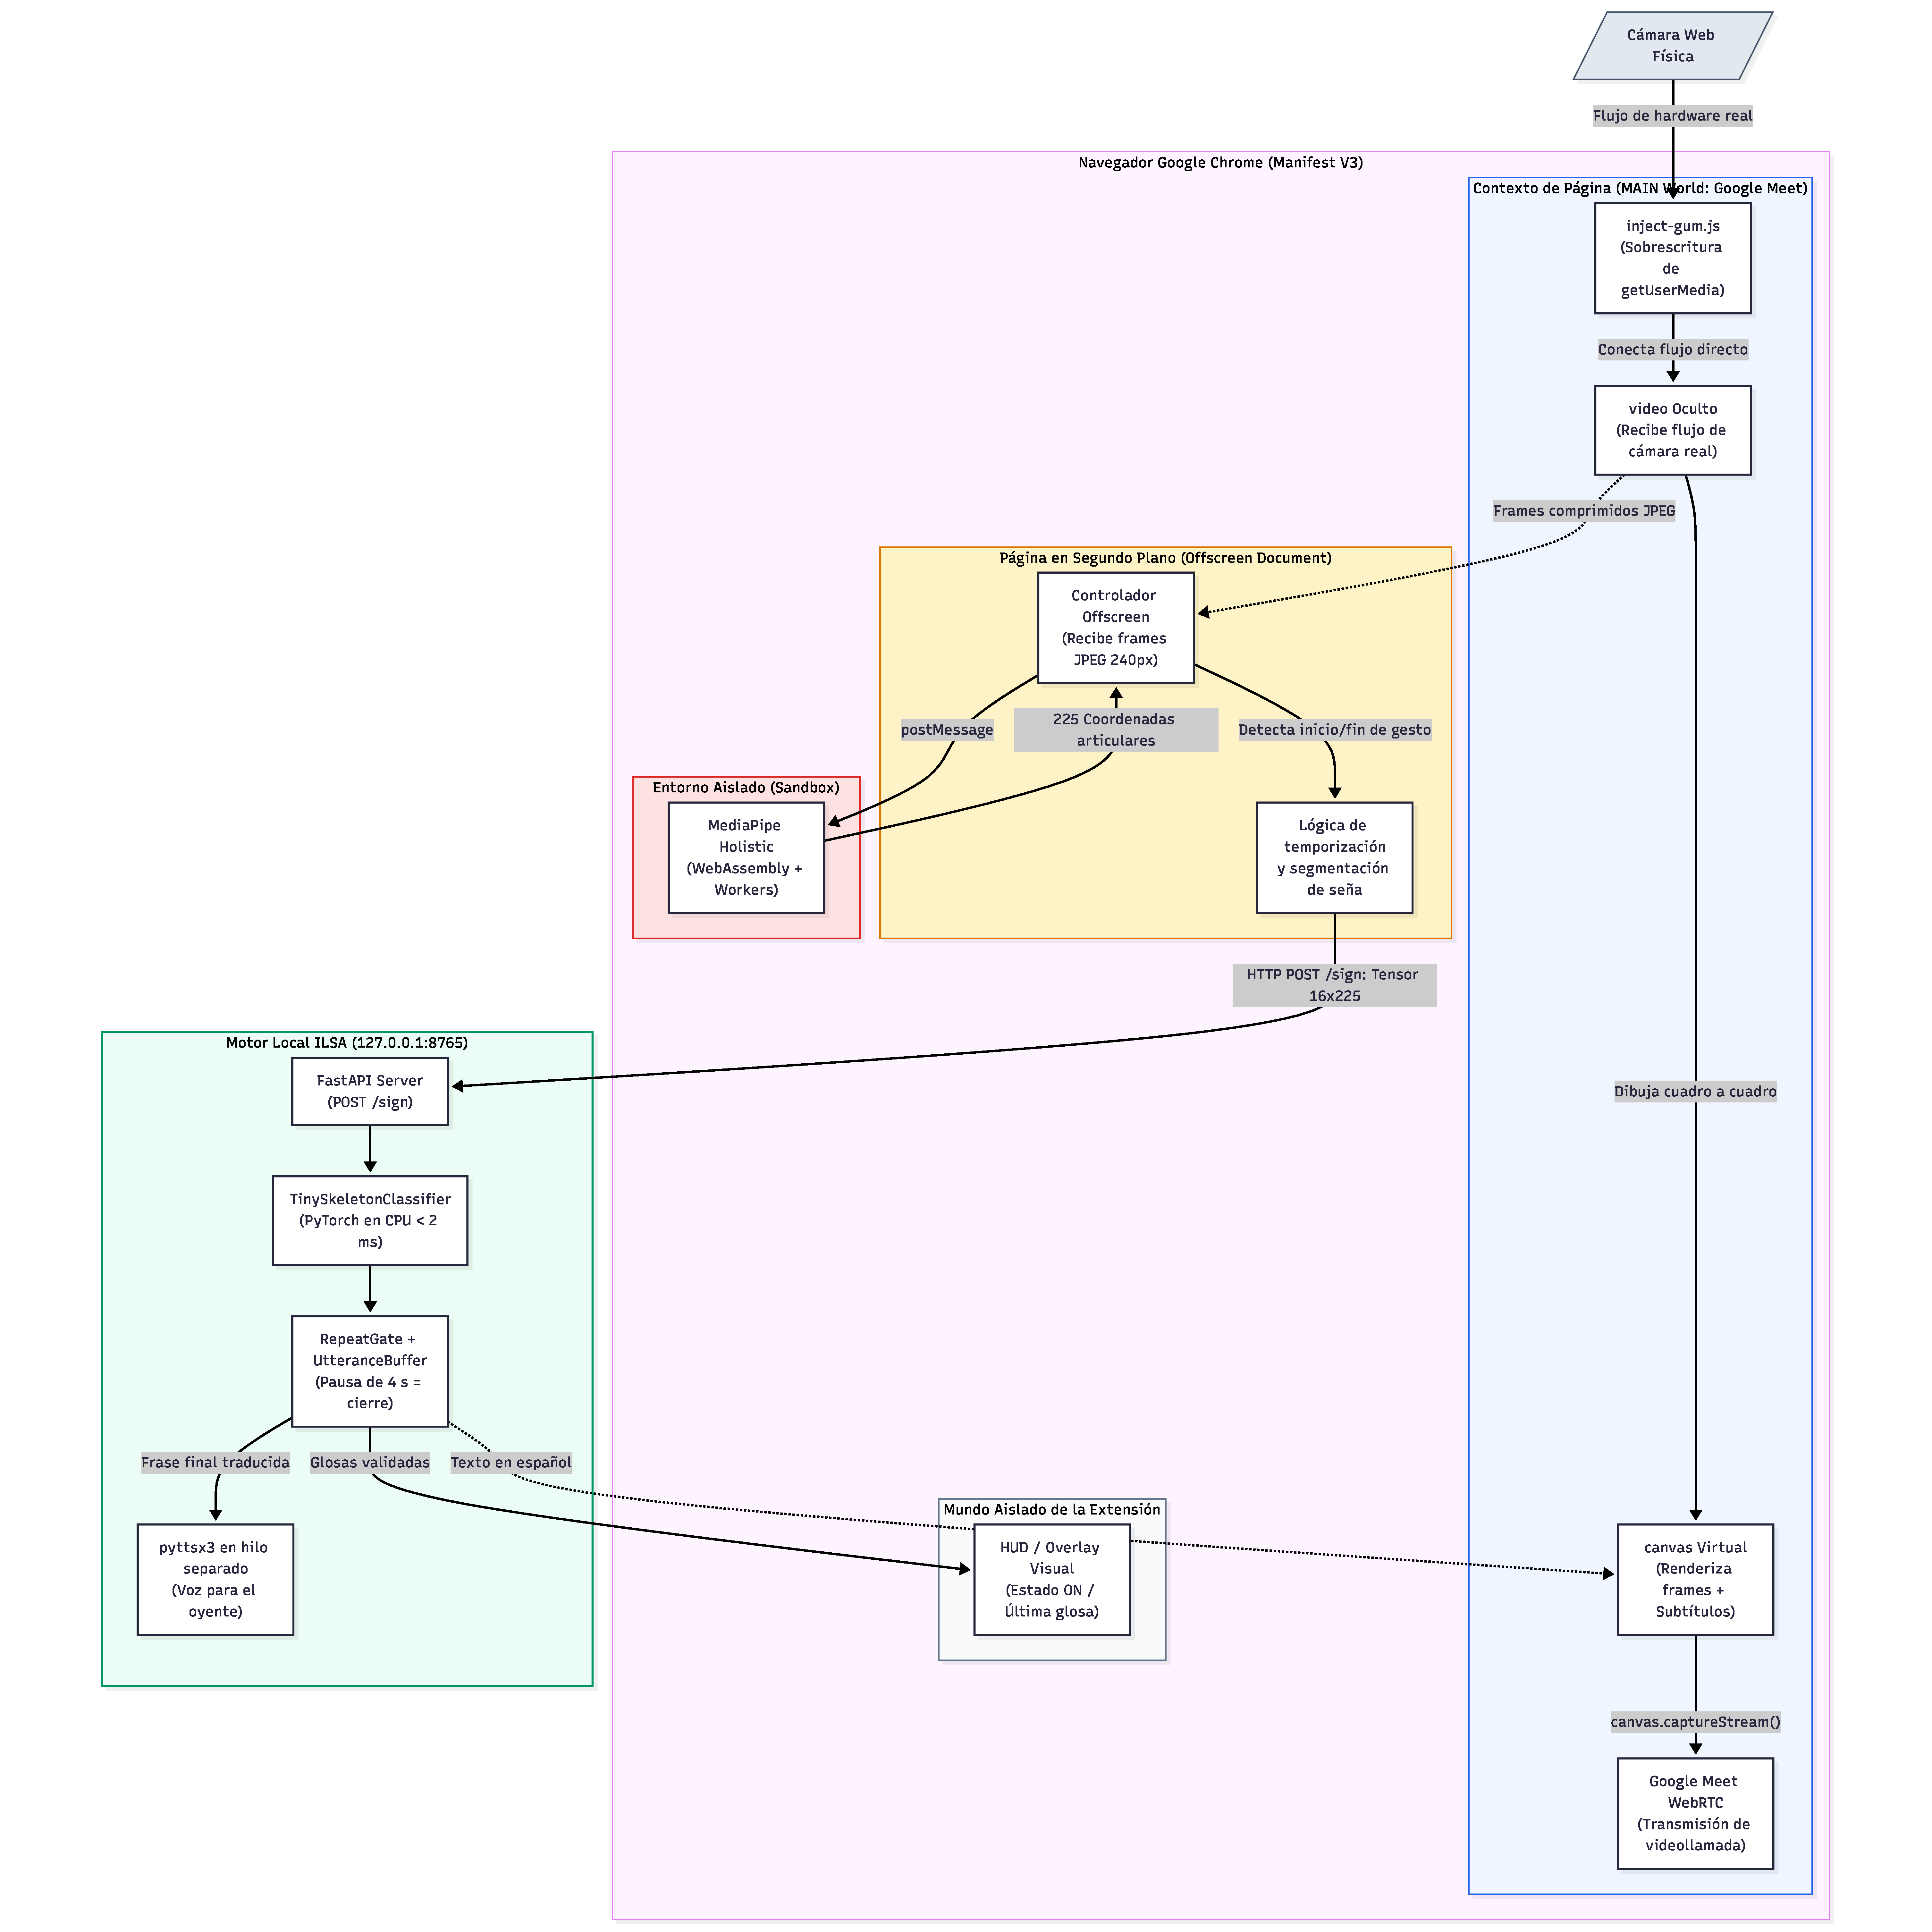
\includegraphics[width=0.85\textwidth,height=0.80\textheight,keepaspectratio]{integracion/Diagrama-arquitectura-extension.pdf}
    \caption{Arquitectura de integración en el navegador: intercepción de la cámara web, derivación de fotogramas al entorno aislado (\textit{offscreen} y \textit{sandbox}) y enlace con el motor local ILSA.}
    \label{fig:arquitectura_extension_meet}
\end{figure}

\paragraph{Página en segundo plano (\textit{offscreen})}
Dado que el \textit{service worker} no puede manipular elementos visuales, creamos un documento sin ventana visible utilizando la API \texttt{chrome.offscreen} \parencite{chrome2024manifestv3}. Su función principal es recibir los cuadros de video en formato comprimido desde la videollamada y coordinar la comunicación con los demás componentes del sistema. Además, para reducir el consumo de CPU y memoria, bajamos la resolución de los cuadros de 320 a 240 píxeles de ancho.

\paragraph{Entorno aislado (\textit{sandbox})}
Para que MediaPipe pudiera ejecutarse sin infringir la política de seguridad del navegador (\textit{Content Security Policy}), declaramos un marco aislado (\textit{sandbox}) en el archivo de manifiesto \parencite{chrome2024manifestv3}. Esta página no tiene acceso directo a las APIs privilegiadas de la extensión ni a la red exterior. Sin embargo, cuenta con los permisos necesarios para instanciar el runtime de WebAssembly y cargar los modelos locales de pose y manos de MediaPipe Holistic \parencite{google2020mediapipe}.

\paragraph{Canal de mensajería y flujo de datos}
El intercambio de información entre estos contextos se organizó mediante un puente de eventos:
\begin{enumerate}
    \item La extensión toma la imagen de la cámara web y la envía al documento \textit{offscreen} como imagen JPEG.
    \item El documento \textit{offscreen} reenvía el cuadro al \textit{sandbox} a través de \texttt{postMessage}.
    \item El entorno \textit{sandbox} procesa la imagen con MediaPipe Holistic y extrae las 225 coordenadas tridimensionales de torso y manos \parencite{google2020mediapipe}.
    \item Los puntos calculados retornan al script \textit{offscreen}, el cual analiza si hay manos activas, recorta la ventana temporal y despacha el vector cinemático al motor local ILSA mediante una petición HTTP POST \parencite{tiangolo2018fastapi}.
\end{enumerate}

Esta separación permitió que Google Meet corriera en su hilo principal sin caídas de cuadros, aislando por completo la carga computacional de la visión artificial dentro de procesos auxiliares del navegador.

\subsection[Intercepción de Media y canvas.captureStream()]{Intercepción de \texttt{getUserMedia} y derivación de flujo vía \texttt{canvas.captureStream()}}

Uno de los mayores desafíos al integrar el sistema en Google Meet fue el acceso a la cámara física. En los navegadores modernos, la API estándar \texttt{navigator.\-mediaDevices.\-getUserMedia} maneja la cámara como un recurso exclusivo: no permite que dos procesos consuman el mismo dispositivo al mismo tiempo sin bloquear el hardware.

En nuestro diseño necesitábamos dos flujos concurrentes: capturar los cuadros de video para extraer los puntos corporales en la extensión y, al mismo tiempo, alimentar la transmisión nativa de la videollamada. Si MediaPipe tomaba el control directo de la cámara, Meet no podía transmitir video; y si Meet la iniciaba primero, el clasificador quedaba bloqueado. 

Para resolver este problema sin alterar el funcionamiento interno de Google Meet, recurrimos a una técnica de intercepción dinámica en el contexto de ejecución principal de la página web (\textit{MAIN world}):

\paragraph{Envoltorio de getUserMedia y desvío a video oculto}
Inyectamos un script (\texttt{inject-gum.js}) que sobrescribe la función \texttt{navigator.mediaDevices.getUserMedia} original. Cuando el motor ILSA está encendido y Meet solicita la cámara, el script intercepta la llamada, obtiene el flujo real del hardware y lo conecta a un elemento \texttt{<video>} invisible en segundo plano. De este modo, la plataforma de videollamada no toma el control del hardware directo.

\paragraph{Generación de flujo sintético con canvas.captureStream()}
Desde ese elemento de video oculto, tomamos los cuadros para derivarlos al flujo de MediaPipe y, en paralelo, los dibujamos cuadro a cuadro sobre un elemento \texttt{<canvas>} virtual. Luego, utilizando el método estandarizado \texttt{canvas.captureStream()} \parencite{w3c2024mediacapture}, sintetizamos un flujo de medios falso (\textit{MediaStream}) que le entregamos a Google Meet como si fuera la cámara web original.

\paragraph{Ventajas del lienzo virtual y gestión de subtítulos}
Esta solución resolvió dos aspectos centrales:
\begin{enumerate}
    \item \textbf{Evitó el bloqueo de hardware:} Ambos procesos comparten el mismo flujo visual sin errores de acceso ni conflictos de permisos.
    \item \textbf{Superposición directa de texto en la señal:} Al controlar el dibujo del lienzo, pudimos pintar las oraciones en español traducidas directamente sobre la parte inferior del video. Así, el interlocutor oyente puede leer los subtítulos en su pantalla sin necesidad de tener instalada nuestra extensión en su navegador.
\end{enumerate}

Para no entorpecer la visión de la llamada, implementamos un temporizador visual: el texto traducido permanece visible durante 8 segundos y desaparece automáticamente. Si llega un enunciado nuevo antes de ese plazo, el reloj se reinicia. Además, si el usuario apaga el motor ILSA, el script retira el interceptor y devuelve el control tradicional de la cámara a Google Meet de inmediato.

\subsection{Motor Local ILSA (FastAPI)}

Para coordinar las tareas locales sin sobrecargar el navegador web, desarrollamos el motor local ILSA (\textit{Intérprete de Lengua de Señas Argentina}). Se trata de una aplicación de escritorio programada en Python que levanta un servidor HTTP local mediante FastAPI y Uvicorn en la dirección de bucle invertido \texttt{127.0.0.1:8765} \parencite{tiangolo2018fastapi}. 

Al diseñar este componente, aprendimos que desacoplar la lógica de clasificación y la síntesis de voz del entorno de Chrome simplifica el mantenimiento y evita problemas de rendimiento en la videollamada. El motor actúa como un orquestador que centraliza cuatro responsabilidades principales:

\paragraph{Recepción de secuencias y ejecución del clasificador}
A través del endpoint \texttt{POST /sign}, el motor recibe los paquetes JSON enviados por la extensión. Cada paquete contiene una secuencia normalizada de 16 fotogramas con 225 coordenadas cinemáticas. El motor convierte estos datos en un tensor de PyTorch con dimensiones $(1, 16, 225)$ y ejecuta la inferencia local del modelo \textit{TinySkeletonClassifier} en CPU en menos de 2\,ms. El resultado se responde inmediatamente a la extensión para actualizar el indicador visual (HUD) en la pantalla del usuario.

\paragraph{Filtrado con RepeatGate y acumulación en UtteranceBuffer}
Cada predicción pasa por la compuerta \texttt{RepeatGate} \parencite{gamma1994design}. Esta clase aplica reglas según el tipo de seña para filtrar rebotes no deseados: admite números repetidos, permite hasta dos letras iguales consecutivas y descarta repeticiones inmediatas en palabras generales. Las glosas aceptadas se van acumulando en el objeto \texttt{UtteranceBuffer}. Si pasan 4 segundos continuos sin actividad gestual, el búfer declara el cierre de la frase y dispara la petición al servidor semántico remoto para obtener la traducción en español.

\paragraph{Manejo de concurrencia y síntesis de voz (pyttsx3)}
Uno de los problemas técnicos que encontramos fue que la librería \texttt{pyttsx3} bloquea el hilo de ejecución mientras pronuncia una frase, además de depender de la arquitectura COM en Windows. Si corríamos la síntesis de voz en el hilo principal de FastAPI, el servidor dejaba de responder peticiones y la cámara se trababa. Para solucionarlo, implementamos una arquitectura concurrente con hilos desacoplados y colas seguras (\texttt{queue.Queue}) \parencite{pressman2014software}. El motor de voz corre en su propio proceso en segundo plano, reproduciendo el audio hacia el oyente sin retrasar la clasificación de nuevas señas.

\paragraph{Empaquetado y distribución ejecutable}
Para que el usuario final no tenga que instalar Python ni configurar entornos virtuales, empaquetamos el backend en un binario ejecutable independiente (\texttt{ILSA.exe}) utilizando PyInstaller. El ejecutable incluye una interfaz gráfica simple donde el usuario puede seleccionar el modo de trabajo (Sordo u Oyente), configurar la mano dominante y encender o apagar el servicio con un solo botón. Al iniciar la sesión, el motor descarga automáticamente la URL pública del servidor semántico desde los lanzamientos de GitHub, permitiendo que la extensión comience a operar en Google Meet de inmediato sin configuraciones manuales de red.
\section{Representación gestual Inversa mediante avatar 3D}
\subsection{Controlador de animaciones esqueléticas por glosas}
\subsection{Mecanismo de contingencia: deletreo manual dactilológico}

\section{Diseño conceptual de la arquitectura escalable en la nube}

La partición funcional adoptada establece que la carga computacional asociada al modelo de lenguaje (el módulo semántico) quede desacoplada de la computadora del usuario y se atienda de manera remota. De este modo, la máquina cliente solo procesa el flujo de cámara y la inferencia gestual liviana, enviando únicamente texto plano (listas de glosas u oraciones) hacia el servidor exterior.

Sin embargo, para llevar esta solución a un entorno de uso masivo con múltiples videollamadas concurrentes, se requiere una infraestructura elástica capaz de procesar turnos simultáneos sin encolamientos ni demoras que corten el ritmo del diálogo. A continuación, se formaliza el diseño conceptual para entornos de producción y se detalla el esquema real con el que se validó el prototipo.

\subsection{Especificación para entornos de producción concurrente}

Para garantizar alta disponibilidad y responder en tiempos medios menores a los 450\,ms por turno frente a múltiples usuarios concurrentes, se proyectó una arquitectura modular basada en microservicios contenerizados y auto-escalado elástico. La topología de recursos y el flujo de balanceo se describen en la Figura~\ref{fig:arquitectura_nube_produccion}.

\begin{figure}[H]
    \centering
    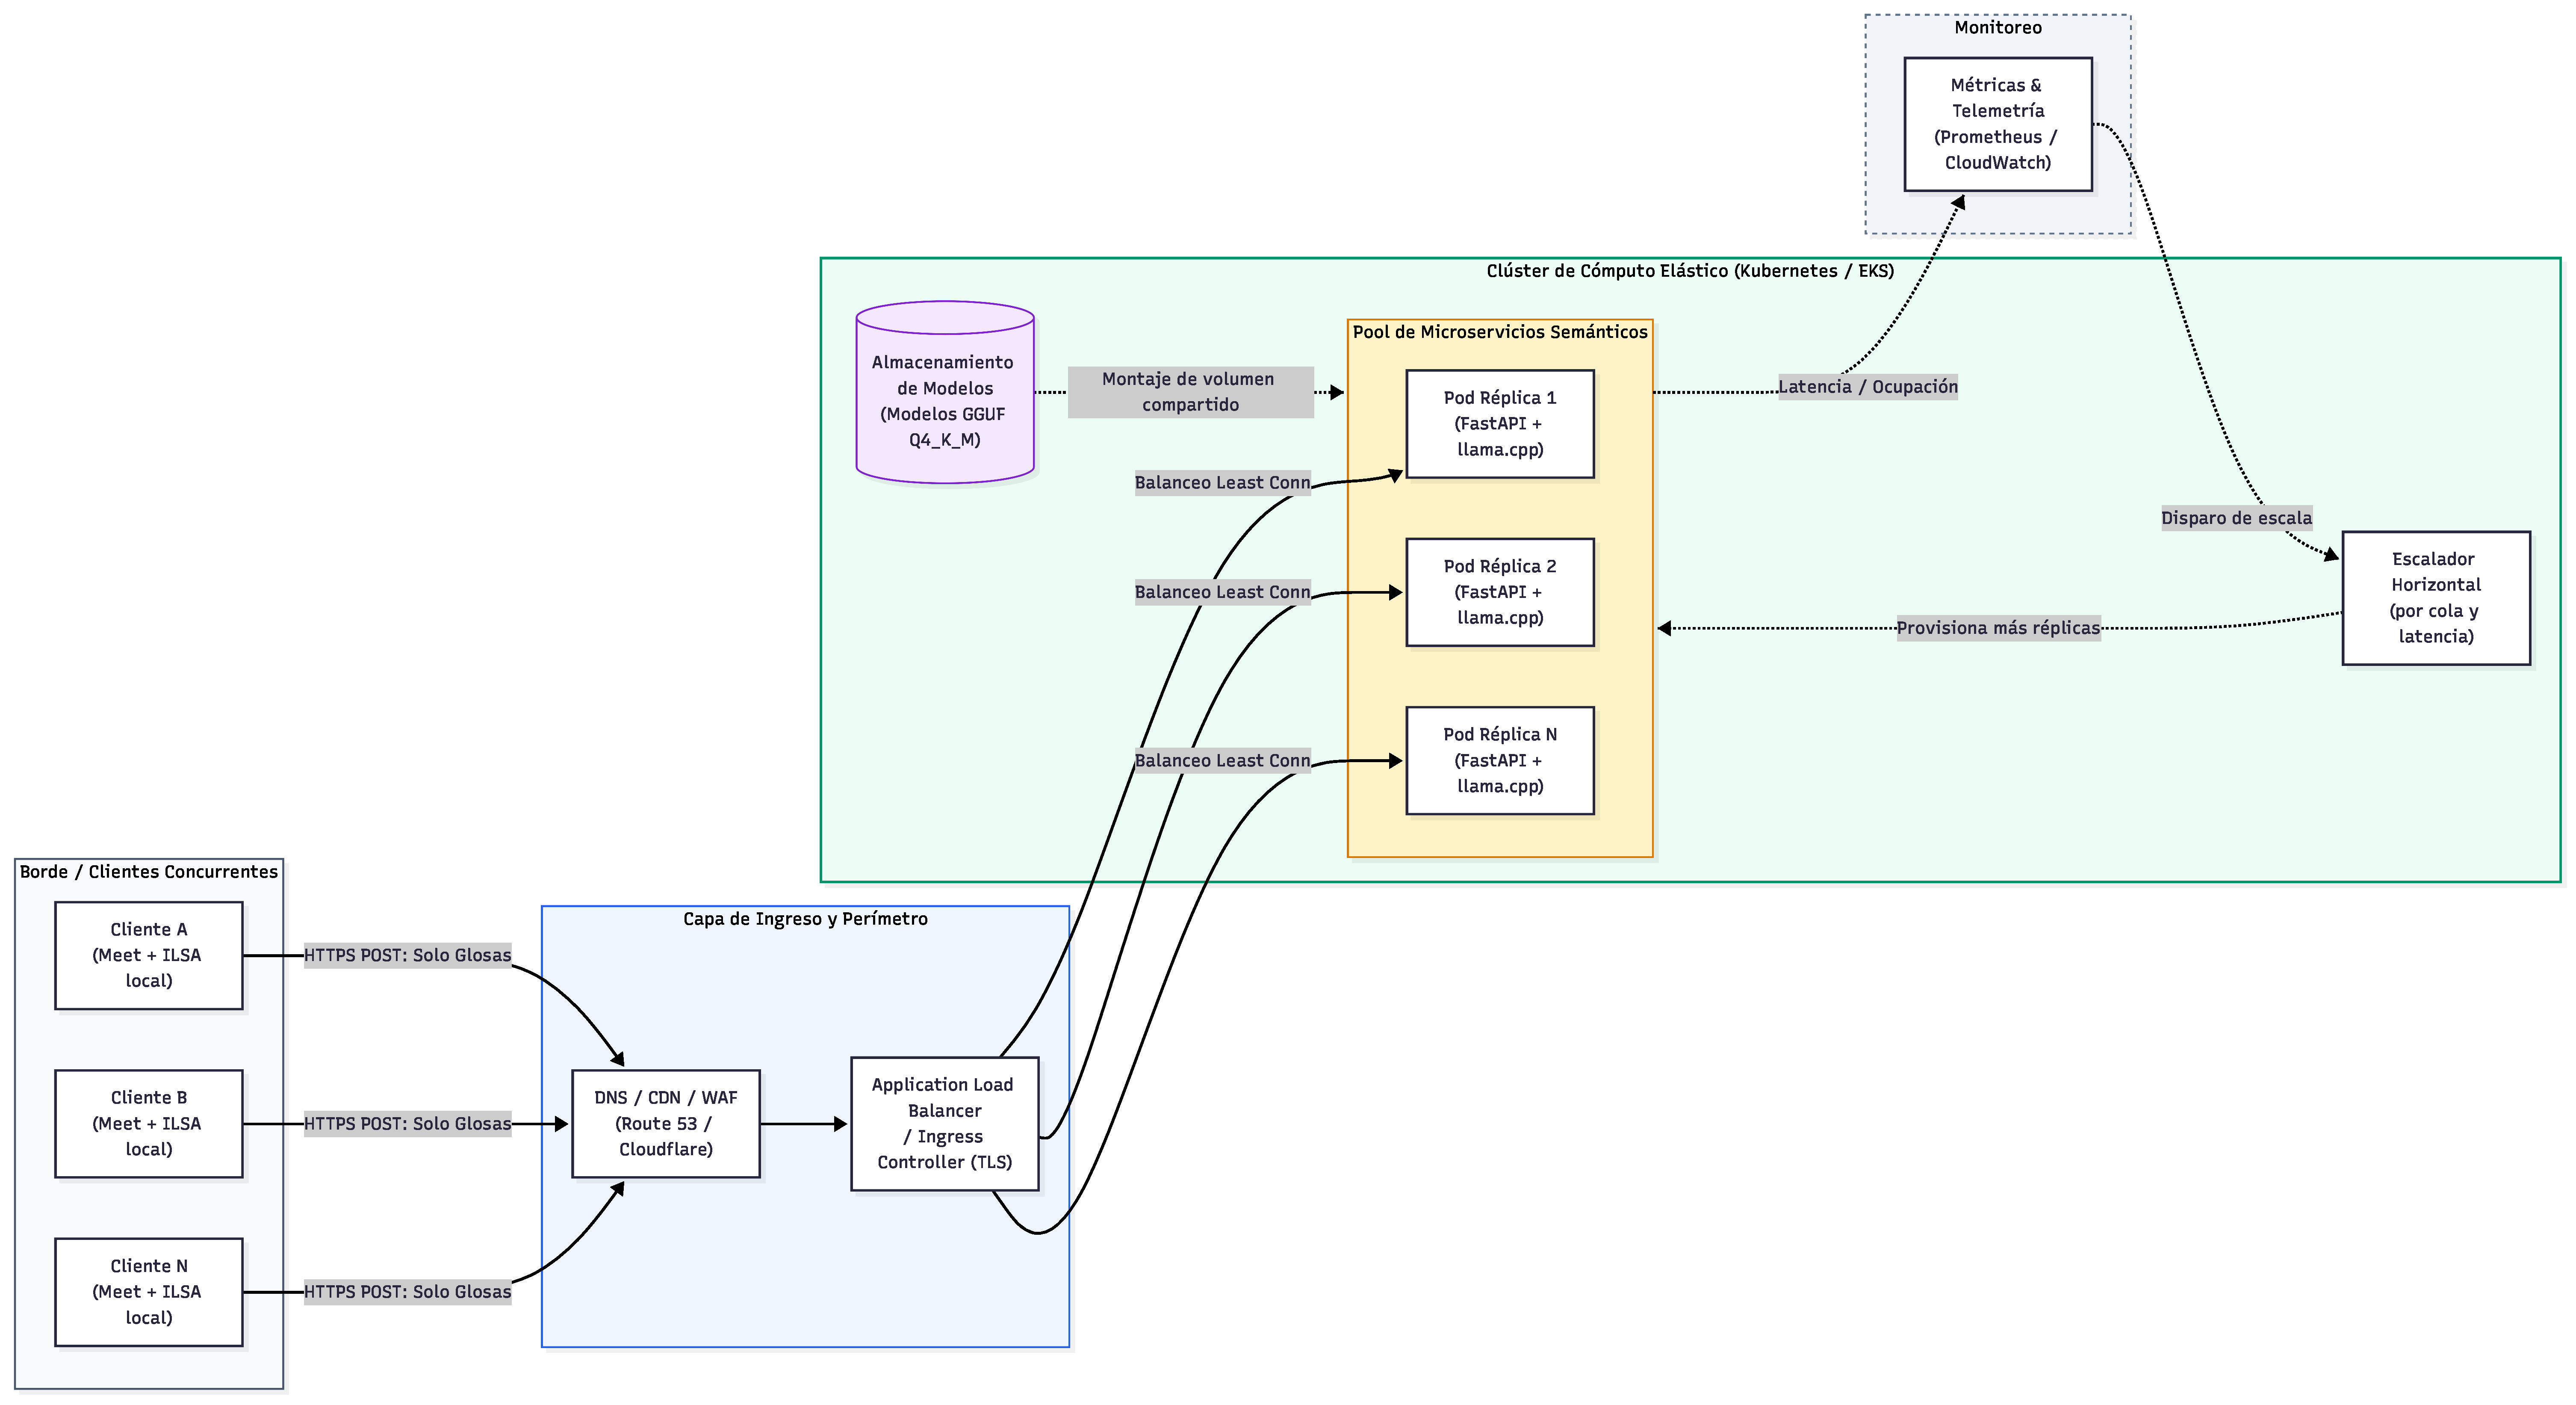
\includegraphics[width=0.95\textwidth]{integracion/Diagrama-arquitcetura-escalable.pdf}
    \caption{Diseño conceptual de la infraestructura en la nube: red perimetral, balanceo de carga y clúster elástico de inferencia semántica con escalado horizontal.}
    \label{fig:arquitectura_nube_produccion}
\end{figure}

El diseño contempla tres capas principales de infraestructura:

\paragraph{Capa de acceso perimetral y balanceo:}
Las solicitudes HTTPS enviadas por las computadoras clientes son recibidas por una capa perimetral que incluye resolución DNS, certificados de seguridad TLS y filtrado de tráfico básico para prevenir saturaciones maliciosas. Detrás de esta capa opera un balanceador de carga (\textit{API Gateway} o \textit{Application Load Balancer}):
\begin{itemize}
    \item Recibe y valida los esquemas JSON de las rutas \texttt{/translate} y \texttt{/hearing}.
    \item Distribuye las peticiones hacia las réplicas del microservicio semántico mediante un criterio de menor número de conexiones activas (\textit{Least Connections}), evitando sobrecargar instancias que se encuentren resolviendo enunciados largos.
\end{itemize}

\paragraph{Clúster de cómputo y escalado elástico:}
El microservicio semántico (desarrollado con FastAPI y el motor de \texttt{llama.cpp}) se empaqueta en imágenes de contenedor Docker \parencite{gerganov2023llamacpp, tiangolo2018fastapi}. Estos contenedores se despliegan sobre un clúster gestionado de Kubernetes (como AWS EKS o equivalente):
\begin{itemize}
    \item \textbf{Almacenamiento compartido de modelos:} Los archivos binarios cuantizados en formato GGUF (Q4\_K\_M) se almacenan en un volumen persistente de solo lectura montado en cada instancia, evitando transferencias repetitivas de red al iniciar nuevos contenedores.
    \item \textbf{Auto-escalado por demanda:} Mediante un controlador de escalado horizontal (HPA), el clúster monitorea la longitud de la cola de peticiones y los tiempos de generación de respuesta. Cuando la cantidad de turnos simultáneos supera el umbral operativo de las réplicas activas, el orquestador provisiona automáticamente nuevos contenedores para absorber el pico de uso.
    \item \textbf{Eficiencia de hardware y costos:} Gracias a la cuantización a 4 bits (GGUF Q4\_K\_M), cada réplica requiere menos de 2\,GB de memoria RAM y puede ejecutarse sobre procesadores estándar en la nube, prescindiendo de servidores dedicados con placa de video (GPU).
\end{itemize}

\paragraph{Monitoreo y telemetría:}
Se prevé un sistema de recopilación de métricas (como Prometheus y Grafana o AWS CloudWatch) para supervisar la latencia por oración, la memoria ocupada por contenedor y la tasa de errores de red, permitiendo calibrar con precisión las reglas de escalado.

\subsection{Instancia de validación del prototipo mediante túnel seguro}

El despliegue comercial continuo de un clúster elástico en proveedores como AWS o Google Cloud Platform implica costos periódicos de infraestructura que no resultaban viables dentro del marco de un Trabajo Final de Grado, tal como quedó establecido en la restricción \texttt{RC-02} de requerimientos.

Para validar el funcionamiento del sistema desacoplado sin incurrir en costos operativos, se implementó una instancia remota de referencia utilizando un túnel seguro cifrado (\textit{Cloudflare Tunnel} o \textit{ngrok}).

\paragraph{Configuración de la instancia de prueba:}
El esquema operativo del prototipo se organizó de la siguiente forma:
\begin{enumerate}
    \item \textbf{Servidor semántico desacoplado:} El servidor se levanto en una computadora separada del equipo donde corría la videollamada. Este proceso levanta el servidor FastAPI, cargando en memoria RAM los binarios cuantizados del traductor gestionados con \texttt{llama-server}.
    \item \textbf{Túnel inverso cifrado:} A través del cliente de ngrok, se estableció un túnel TLS saliente que generó una URL pública con HTTPS (por ejemplo, \texttt{https://ilsa-semantic.trycloudflare.com}). Esto permitió exponer el servicio a Internet de forma segura sin requerir una IP pública fija ni configurar redirecciones de puertos en el rúter.
    \item \textbf{Conexión del cliente local:} El motor ILSA en la computadora del usuario lee la URL remota mediante la variable de configuración \texttt{SEMANTIC\_URL} o la consulta al iniciar la aplicación. Al detectar el fin de una frase de señas, despacha la lista de glosas por la red pública hacia dicho punto de acceso.
\end{enumerate}

\paragraph{Validez técnica de las pruebas}
Este esquema reprodujo con exactitud el comportamiento que tendría el sistema en un entorno de producción real:
\begin{itemize}
    \item Incorporó los retardos típicos de una red de telecomunicaciones residencial (latencias de subida y bajada, fluctuaciones de conexión y negociación TLS).
    \item Verificó que los contratos de datos y la serialización JSON funcionaran de manera consistente a través de Internet.
    % TODO; Chequear metricas
    \item Demostró que la computadora cliente de 8\,GB de RAM se mantuvo liberada del consumo de memoria y CPU del modelo de lenguaje, garantizando que Google Meet y MediaPipe operaran a 30 FPS continuos sin caídas de rendimiento \parencite{google2020mediapipe}.
\end{itemize}

De esta manera, se comprobó la viabilidad del modelo híbrido cliente-nube, dejando la aplicación preparada para migrar a una infraestructura en la nube simplemente actualizando la dirección URL del servicio semántico.


% ====================================================================
\chapter{Experimentación, Resultados y Discusión}
% ====================================================================

\section{Corpus y metodología de adquisición de Datos de LSA}
\subsection{Definición y validación del vocabulario de 100 clases}
\subsection{Protocolo de grabación y curación del dataset propio}


\section{Evaluación empírica del clasificador gestual}
\subsection{Métricas offline vs. rendimiento en cámara real}
\subsection{Impacto de la resolución temporal: 16 vs. 32 fotogramas}
\subsection{Búsqueda automatizada de hiperparámetros con Optuna y Análisis de sobreajuste}
\subsection{Diagnóstico de confusiones mediante feature engineering y separabilidad}
\subsection{Impacto cuantitativo de la corrección de aspect ratio}
\subsection{Desempeño final del clasificador baseline en vivo}

\section{Evaluación de los módulos de traducción semántica}
\subsection{Benchmark comparativo de modelos SLM (Familias Qwen2.5, Llama 3.2 y SmolLM2)}
\subsection{Evaluación cuantitativa: BLEU, ROUGE-L, METEOR y exactitud}
\subsection{Análisis de simetría en el aprendizaje: traducción directa vs. estructuración inversa}
\subsection{Compromiso entre calidad lingüística y latencia de inferencia}

\section{Evaluación del sistema integrado y rendimiento en tiempo real}
\subsection{Validación funcional de extremo a extremo en videollamadas reales}
\subsection{Análisis de latencias totales por etapa del pipeline}
\subsection{Consumo de recursos de hardware: máquina de desarrollo vs. máquina objetivo}
\subsection{Discusión técnica y lecciones de ingeniería aprendidas}



% ====================================================================
\chapter{Conclusiones y trabajo futuro}
% ====================================================================

\section{Conclusiones}
\subsection{Cumplimiento de objetivos del proyecto}
\subsection{Aportes técnicos y de accesibilidad}
\subsection{Impacto social en el marco de la Ley 27.710}

\section{Trabajo futuro}
\subsection{Implementación física del clúster semántico escalable}
\subsection{Expansión del corpus multiseñante y mitigación de variabilidad}
\subsection{Incorporación de rasgos no manuales (expresiones faciales)}
\subsection{Generalización a nuevas plataformas de comunicación virtual}


% --- Bibliografía ---
\printbibliography

% --- Apéndices ---
\appendix
\include{capitulos/apendice_a_vocabulario}
\include{capitulos/apendice_b_configuraciones}


\end{document}